\subsection{\vdmh}
\Opensolutionfile{ans}[ans/DA-CD4-VD]
\begin{vd}[TN2024-102]%[2H2N2-3]
    Trong không gian $Oxyz$, cho hai véc-tơ $\overrightarrow{a}=(2; 3;-1)$ và $\overrightarrow{b}=(-3; 2;-4)$. Véc-tơ $\overrightarrow{a}+\overrightarrow{b}$ có tọa độ là
    \choice
    {$(-5;-1;-3)$}
    {\True $(-1; 5;-5)$}
    {$(-1;-5; 5)$}
    {$(1;-5; 5)$}
%    \loigiai
%    {
%        Hoành độ của véc-tơ $\overrightarrow{a} + \overrightarrow{b}$ là $2+(-3) = -1$.\\
%        Tung độ của véc-tơ $\overrightarrow{a} + \overrightarrow{b}$ là $3+2 = 5$.\\
%        Cao độ của véc-tơ $\overrightarrow{a} + \overrightarrow{b}$ là $-1+(-4) = -5$.\\
%        Vậy véc-tơ $\overrightarrow{a}+\overrightarrow{b}$ có tọa độ là $(-1;5;-5)$.
%    }
\end{vd}
\begin{vd}[CHUYÊN PHAN BỘI CHÂU - NGHỆ AN]%[2H2H2-3]
    Trong không gian $Oxyz$, cho ba vecto $\overrightarrow{a}=(2;-1;0)$, $\overrightarrow{b}=(-1;-3;2)$, $\overrightarrow{c}=(-2;-4;-3)$. Tọa độ của vecto $\overrightarrow{u}=2\overrightarrow{a}-3\overrightarrow{b}+\overrightarrow{c}$ là
    \choice
    {$(3;7;9)$}
    {$(-3;-7;-9)$}
    {\True $(5;3;-9)$}
    {$(-5;-3;9)$}
    \loigiai{Ta có $\heva{&2\overrightarrow{a}=(4;-2;0)\\&3\overrightarrow{b}=(-3;-9;6)\\&\overrightarrow{c}=(-2;-4;-3)}\Rightarrow\overrightarrow{u}=2\overrightarrow{a}-3\overrightarrow{b}+\overrightarrow{c}=(5;3;-9)$.}
\end{vd}
\begin{vd}[SỞ YÊN BÁI]%[2H2N1-3]
    Trong không gian $Oxyz$ , cho hai vectơ $\overrightarrow {u}=\overrightarrow {i}+3\overrightarrow {j}-2\overrightarrow {k} $ và $\overrightarrow {v}=\left(2;-1;1\right)$. Tích vô hướng $\overrightarrow {u} \cdot \overrightarrow {v}$ bằng
    \choice
    {$\overrightarrow {u} \cdot \overrightarrow {v}=-12$}
    {$\overrightarrow {u} \cdot \overrightarrow {v}=5\sqrt 2 $}
    {\True $\overrightarrow {u} \cdot \overrightarrow {v}=-3$}
    {$\overrightarrow {u} \cdot \overrightarrow {v}=2\sqrt{21}$}
    \loigiai{
        Ta có $\overrightarrow {u}=\left(1;3;-2\right)$ ; $\overrightarrow {v}=\left(2;-1;1\right)$ nên $\overrightarrow {u} \cdot \overrightarrow {v}=1\cdot 2+\cdot \left(-1\right)+\left(-2\right)\cdot 1=-3$.}
\end{vd}
\begin{vd}[SỞ TUYÊN QUANG]%[2H2H2-3]
    Trong không gian với hệ trục tọa độ $Oxyz$, cho hai điểm $A(1;-3;1)$, $B(3;0;-2)$. Độ dài đoạn thẳng $AB$ bằng
    \choice
    {\True $\sqrt{22}$}
    {$\sqrt{26}$}
    {$26$}
    {$22$}
    \loigiai
    {
        Độ dài đoạn thẳng $AB=\sqrt{(3-1)^2+(0+3)^2+(-2-1)^2}=\sqrt{22}$.	
    }
\end{vd}
\begin{vd}[TN2024-102]%[2H5N2-3]
    Trong không gian $Oxyz$, cho điểm $A(1;2;-1)$ và mặt phẳng $(P)\colon 2x-z+1=0$. Đường thẳng đi qua $A$ và vuông góc với $(P)$ có phương trình là
    \choice
    {$\heva{&x=-1+2t\\&y=-2\\&z=1-t}$}
    {$\heva{&x=-2+t\\&y=2t\\&z=-1-t}$}
    {\True $\heva{&x=1+2t\\&y=2\\&z=-1-t}$}
    {$\heva{&x=1+2t\\&y=2-t\\&z=-1+t}$}
    \loigiai{
        Đường thẳng $d$ vuông góc với $(P)$ nên ta chọn $\vec{u}_d=\vec{n}_{(P)}=(2;0;-1)$. \\
        Phương trình đường thẳng $d$ cần tìm là $\heva{&x=1+2t\\&y=2\\&z=-1-t}$.
    }
\end{vd}
\begin{vd}[CHUYÊN PHAN BỘI CHÂU - NGHỆ AN]%[2H2N2-2]
    Trong không gian $Oxyz$, hình chiếu vuông góc của điểm $M(-2;3;4)$ lên trục $Oy$ là điểm nào?
    \choice
    {$M_1(-2;0;0)$}
    {\True $M_2(0;3;0)$}
    {$M_3(0;0;4)$}
    {$M_4(-2;0;4)$}
%    \loigiai{Hình chiếu vuông góc của điểm $M(-2;3;4)$ lên trục $Oy$ là điểm $M_2(0;3;0)$.}
\end{vd}
\begin{vd}%[2H2H2-2]
    Trong không gian $Oxyz$, cho hai điểm $A (2; 3 ; -2 )$ và $B (-2; 4; 1 )$. Biết $B$ là trung điểm của đoạn thẳng $AC$. Khi đó, tọa độ của điểm $C$ là
    \choice
    {$ (2; 5; 0 )$}
    {$ (-4; 1; 3 )$}
    {$ (6; 2; -5 )$}
    {\True $ (-6; 5; 4 )$}
    \loigiai
    {
        Gọi $C (a; b; c )$. \\
        Vì $B$ là trung điểm của đoạn thẳng $AC$ nên
        $\heva{
            &-2=\dfrac{2+a}{2}  \\
            &4=\dfrac{3+b}{2}  \\
            &1=\dfrac{-2+c}{2}  \\
        }$
        $\Leftrightarrow 
        \heva{
            &a=-6  \\
            &b=5  \\
            &c=4  \\
        }$.\\
        Vậy $C (-6; 5; 4 )$.
    }
\end{vd}
\begin{vd}%[2H2H2-2]
    Trong không gian với hệ tọa độ $Oxyz$, cho tam giác $ABC$ biết $A(2;4;-3)$ và $\overrightarrow{AB}=(-3;-1;1)$, $\overrightarrow{AC}=(2;-6;6)$. Khi đó tọa độ trọng tâm $G$ của tam giác $ABC$ là:
    \choice
    {\True $G \left({ \dfrac{5}{3}; \dfrac{5}{3};- \dfrac{2}{3}} \right)$}
    {$G \left({ \dfrac{5}{3};- \dfrac{5}{3}; \dfrac{2}{3}} \right)$}
    {$G \left({- \dfrac{5}{3}; \dfrac{5}{3}; \dfrac{2}{3}} \right)$}
    {$G \left({ \dfrac{5}{3}; \dfrac{5}{3}; \dfrac{2}{3}} \right)$}
    \loigiai
    {
        Ta có : $A(2;4;-3)$ và $\overrightarrow{AB}=(-3;-1;1)$, suy ra $B (-1;3;-2 )$.\\
        $A(2;4;-3)$ và $\overrightarrow{AC}=(2;-6;\text{ }6)$, suy ra $C (4;-2;3 )$.\\
        $G$ là trọng tâm của tam giác $ABC$ nên ta có: \\
        $\heva{
            {{x}_{G}}= \dfrac{2-1+4}{3}= \dfrac{5}{3} \\ 
            {{y}_{G}}= \dfrac{4+3-2}{3}= \dfrac{5}{3} \\ 
            {{z}_{G}}= \dfrac{-3-2+3}{3}=- \dfrac{2}{3} \\ 
        }
        \Rightarrow G \left({ \dfrac{5}{3}; \dfrac{5}{3};- \dfrac{2}{3}} \right)$.
    }
\end{vd}
\begin{vd}%[2H2H2-2]
    Trong không gian $Oxyz$, cho tam giác $ABC$ có các điểm $A(1; 0; 3)$, $B(2; 3; -4)$ và $C(-3; 1; 2)$. Tìm toạ độ điểm $D$ sao cho tứ giác $ABCD$ là hình bình hành. 
    \choice
    {\True $(-4; -2; 9)$}
    {$(4; 2; 9)$}
    {$(-2; 4; -5)$}
    {$(6; 2; -3)$}
    \loigiai{
        Gọi $D(x; y; z) \Rightarrow \overrightarrow{CD}=(x+3; y-1; z-2)$ và $\overrightarrow{BA}=(-1; -3; 7)$.\\
        Tứ giác $ABCD$ là hình bình hành khi và chỉ khi $$\overrightarrow{BA}=\overrightarrow{CD} \Leftrightarrow\heva{&x+3=-1 \\&y-1=-3 \\ &z-2=7} \Leftrightarrow \heva{&x=-4 \\&y=-2 \\&z=9} \Rightarrow C(-4; -2; 9).$$}
\end{vd}
\begin{vd}%[2H2H2-2]
    Trong không gian $Oxyz$, cho điểm $A(1; 2; 3)$. Tìm tọa độ $A'$ là điểm đối xứng với $A$ qua trục $Oy$.
    \choice
    {$A'(1; -2; 3)$}
    {$A'(1; 2; -3)$}
    {$A'(-1; 2; 3)$}
    {\True $A'(-1; 2; -3)$}
%    \loigiai{
%        Gọi $H$ là hình chiếu vuông góc của $A(1; 2; 3)$ lên $Oy$. Suy ra $H(0; 2; 0)$. \\
%        Khi đó $H$ là trung điểm đoạn $AA'$.\\
%        Suy ra
%        $\heva{&x_{A'}=2 x_H-x_A=-1 \\& y_{A'}=2 y_H-y_A=2 \\& z_{A'}=2 z_H-z_A=-3} \Rightarrow A'(-1; 2; -3)$.
%    }
\end{vd}
\begin{vd}[SỞ YÊN BÁI]%[2H5N1-2]
    Cho mặt phẳng $(P)$ có phương trình $2x-y+z-2=0$. Điểm nào dưới đây thuộc mặt phẳng $(P)$?
    \choice
    {\True $N(1;-1;-1)$}
    {$M(1;1;-1)$}
    {$P(2;-1;-1)$}
    {$Q(1;-2;2)$}
%    \loigiai{
%        Ta có $2\cdot 1-\left(-1\right)+\left(-1\right)-2=0$ nên $N\left(1;-1;-1\right)$ thuộc mặt phẳng $(P)$.}
\end{vd}
\begin{vd}[TN2024-102]%[2H5N1-3]
    Trong không gian $Oxyz$, mặt phẳng đi qua điểm $M(3;4;-2)$ và vuông góc với trục $Oz$ có phương trình là
    \choice
    {$y-4=0$}
    {$x-3=0$}
    {$x+y+z-5=0$}
    {\True $z+2=0$}
    \loigiai{
        Ta có véc-tơ đơn vị của trục $Oz$ là $\overrightarrow{k}=(0;0;1)$.\\
        Mặt phẳng qua $M(3;4;-2)$ và nhận véc-tơ $\overrightarrow{k}=(0;0;1)$ là véc-tơ pháp tuyến nên có phương trình là
        $$0\cdot(x-3)+0\cdot(y-4)+1\cdot(z+2)=0\Leftrightarrow z+2=0.$$
    }
\end{vd}
\begin{vd}[TN2025-0101]%[2H5N1-3]
    Trong không gian $Oxyz$, mặt phẳng đi qua điểm $A(2;1;-4)$ nhận $\overrightarrow{n}=(3;2;-1)$ làm một véc-tơ pháp tuyến có phương trình là
    \choice
    {\True $3(x-2)+2(y-1)-(z+4)=0$}
    {$2(x+3)+(y+2)-4(z-1)=0$}
    {$3(x+2)+2(y+1)-(z-4)=0$}
    {$2(x-3)+(y-2)-4(z+1)=0$}
    \loigiai{
        Mặt phẳng đi qua điểm $A(2;1;-4)$ nhận $\overrightarrow{n}=(3;2;-1)$ làm một véc-tơ pháp tuyến có phương trình là 
        $$3(x-2)+2(y-1)-(z+4)=0.$$
    }
\end{vd}
\begin{vd}[SỞ HẬU GIANG]%[2H5N1-3]
    Trong không gian với hệ trục tọa độ $Oxyz$, phương trình của mặt phẳng $(P)$ đi qua 3 điểm $E(2;0;0)$, $F(0;-3;0)$ và $K(0;0;5)$ là
    \choice
    {\True $\dfrac{x}{2}+\dfrac{y}{-3}+\dfrac{z}{5}=1$}
    {$\dfrac{x}{2}+\dfrac{y}{-3}+\dfrac{z}{5}=-1$}
    {$2x-3y+5z-30=0$}
    {$\dfrac{x}{2}+\dfrac{y}{-3}+\dfrac{z}{5}=0$}
    \loigiai
    {Mặt phẳng $(P)$ đi qua $3$ điểm $E(2;0;0)$, $F(0;-3;0)$ và $K(0;0;5)$ nên có phương trình theo đoạn chắn là $\dfrac{x}{2}+\dfrac{y}{-3}+\dfrac{z}{5}=1$.
    }
\end{vd}
\begin{vd}[SỞ VĨNH PHÚC]%[2H5V1-6]
    Trong không gian $Oxyz$ cho hai mặt phẳng $(P)\colon mx+2y+mz-12=0$ và $(Q)\colon x+my+z+2025=0$. Có bao nhiêu giá trị của $m$ sao cho góc giữa hai mặt phẳng $(P)$ và $(Q)$ bằng $45^\circ$?
    \choice
    {$3$}
    {\True $4$}
    {$2$}
    {$0$}
    \loigiai{
        Hai mặt phẳng $(P)$ và $(Q)$ lần lượt có véc-tơ pháp tuyến là $\overrightarrow{n}_{P}=(m;2;m)$; $\overrightarrow{n}_{Q}=\left(1; m; 1\right)$.\\
        Ta có $$\cos\left((P);(Q)\right)=\left|\cos\left(\overrightarrow{n}_{P}, \overrightarrow{n}_{Q}\right)\right|=\dfrac{\left|\overrightarrow{n}_{P}\cdot \overrightarrow{n}_{Q}\right|}{\left|\overrightarrow{n}_{P}\right|\cdot \left|\overrightarrow{n}_{Q}\right|}=\dfrac{\left| m\cdot 1+2\cdot m+m\cdot 1\right|}{\sqrt{m^2+2^2+m^2}\cdot \sqrt{1^2+m^2+1^2}}.$$
        Theo đề, góc giữa hai mặt phẳng $(P)$ và $(Q)$ bằng $45^\circ$ nên ta có
        \allowdisplaybreaks
        \begin{eqnarray*}
            \cos 45^\circ=\dfrac{\left| 4\cdot m\right|}{\sqrt{2\cdot m^2+4}\cdot \sqrt{m^2+2}} 
            &\Leftrightarrow&\dfrac{\sqrt{2}}{2}=\dfrac{\left| 4m\right|}{\sqrt{2m^2+4}\cdot \sqrt{m^2+2}}\\ 
            &\Leftrightarrow&\dfrac{\sqrt{2}}{2}=\dfrac{\left| 4m\right|}{\sqrt{2}\sqrt{m^2+2}\cdot \sqrt{m^2+2}}\\ 
            &\Leftrightarrow&{m^2}+2=\left| 4m\right|\\ 
            &\Leftrightarrow&{\left(m^2+2\right)^2}=16m^2\\ 
            &\Leftrightarrow&{m^4}-12m^2+4=0\\
            &\Leftrightarrow&\hoac{&m^2=6+4\sqrt{2}\\&m^2=6-4\sqrt{2}}\\
            &\Leftrightarrow& \hoac{&
                m=\pm\sqrt{6+4\sqrt{2}}\\&
                m=\pm\sqrt{6-4\sqrt{2}}.}	
        \end{eqnarray*}
        Vậy có $4$ giá trị $m$ để góc giữa hai mặt phẳng $(P)$ và $(Q)$ bằng $45^\circ$.}
\end{vd}
\begin{vd}[TN2024-102]%[2H5N2-3]
    Trong không gian $Oxyz$, cho điểm $A(1;2;-1)$ và mặt phẳng $(P)\colon 2x-z+1=0$. Đường thẳng đi qua $A$ và vuông góc với $(P)$ có phương trình là
    \choice
    {$\heva{&x=-1+2t\\&y=-2\\&z=1-t}$}
    {$\heva{&x=-2+t\\&y=2t\\&z=-1-t}$}
    {\True $\heva{&x=1+2t\\&y=2\\&z=-1-t}$}
    {$\heva{&x=1+2t\\&y=2-t\\&z=-1+t}$}
    \loigiai{
        Đường thẳng $d$ vuông góc với $(P)$ nên ta chọn $\vec{u}_d=\vec{n}_{(P)}=(2;0;-1)$. \\
        Phương trình đường thẳng $d$ cần tìm là $\heva{&x=1+2t\\&y=2\\&z=-1-t}$.
    }
\end{vd}

\begin{vd}[TN2025-0101]%[2H5N2-2]
    Trong không gian $Oxyz$, cho đường thẳng $(d)\colon \dfrac{x-3}{4}=\dfrac{y+2}{-5}=\dfrac{z-1}{2}$. Véc-tơ nào sau đây là một véc-tơ chỉ phương của đường thẳng $(d)$?
    \choice
    {$\overrightarrow{v}_3=(4; 5; 2)$}
    {$\overrightarrow{v}_1=(3;-2; 1)$}
    {$\overrightarrow{v}_4=(3; 2; 1)$}
    {\True $\overrightarrow{v}_2=(4;-5; 2)$}
%    \loigiai{
%        Từ phương trình chính tắc của đường thẳng $d$, ta thấy $\overrightarrow{v}_2=(4;-5; 2)$ là một véc-tơ chỉ phương của đường thẳng $(d)$.
%    }
\end{vd}
\begin{vd}[TN2024-102]%[2H5N2-2]
    Trong không gian $Oxyz$, cho đường thẳng $d\colon \dfrac{x+1}{1} =\dfrac{y-2}{-1} =\dfrac{z}{-3}$. Véc-tơ nào dưới đây là một véc-tơ chỉ phương của $d$?
    \choice
    {$\overrightarrow{u}_2=(-1; 2; 0)$}
    {\True $\overrightarrow{u}_3=(1;-1; -3)$}
    {$\overrightarrow{u}_4=(1; 1; 3)$}
    {$\overrightarrow{u}_1=(1; 2; 0)$}
%    \loigiai
%    {
%        Một véc-tơ chỉ phương của đường thẳng $d\colon \dfrac{x+1}{1} =\dfrac{y-2}{-1} =\dfrac{z}{-3}$ là $\overrightarrow{u}_3=(1;-1; -3)$.
%    }
\end{vd}
\begin{vd}[KHTN-HÀ NỘI - LẦN 2]%[2H5N2-1]
    Cho đường thẳng $d\colon \dfrac{x+1}{2}=\dfrac{y-1}{-1}=\dfrac{z+2}{-2}$. Điểm nào dưới đây thuộc đường thẳng $d$.
    \choice
    {$A(-1;1;2)$}
    {$B(1;-1;2)$}
    {$C(1;0;4)$}
    {\True $D(1;0;-4)$}
%    \loigiai{
%        Thay tọa độ $D(1;0;-4)$ vào phương trình chính tắc của $d$ ta được
%        $\dfrac{1+1}{2}=\dfrac{0-1}{-1}=\dfrac{-4+2}{-2}$ (Đúng).\\
%        Suy ra điểm $D(1;0;-4)$ thuộc đường thẳng $d$.
%    }
\end{vd}
\begin{vd}[CHUYÊN PHAN BỘI CHÂU - NGHỆ AN]%[2H5H2-3]
    Trong không gian $Oxyz$, cho hai điểm $M(-1;-1;2)$ và $N(1;3;4)$. Đường thẳng $MN$ có phương trình chính tắc là
    \choice
    {$\dfrac{x-1}{2}=\dfrac{y-1}{2}=\dfrac{z+2}{1}$}
    {$\dfrac{x+1}{2}=\dfrac{y+3}{4}=\dfrac{z+4}{2}$}
    {$\dfrac{x-1}{2}=\dfrac{y-1}{4}=\dfrac{z+2}{2}$}
    {\True $\dfrac{x+1}{1}=\dfrac{y+1}{2}=\dfrac{z-2}{1}$}
%    \loigiai{Ta có $\overrightarrow{MN}=(2;4;2)=2(1;2;1)$.\\
%        Đường thẳng $MN$ đi qua điểm $M(-1;-1;2)$ nhận véc-tơ $\overrightarrow{u}=(1;2;1)$ làm véc-tơ chỉ phương nên có phương trình chính tắc $\dfrac{x+1}{1}=\dfrac{y+1}{2}=\dfrac{z-2}{1}$.}
\end{vd}
\begin{vd}[MH-2025]%[2H5N2-3]
    Trong không gian với hệ trục tọa độ $Oxyz$, phương trình của đường thẳng đi qua điểm $M(1;-3;5)$ và có một vectơ chỉ phương $\overrightarrow{u}(2;-1;1)$ là:
    \choice
    {$\dfrac{x-1}{2} = \dfrac{y+3}{-1} = \dfrac{z-5}{1}$}
    {$\dfrac{x+1}{2} = \dfrac{y+3}{-1} = \dfrac{z+5}{1}$}
    {\True $\dfrac{x-1}{2} = \dfrac{y+3}{1} = \dfrac{z-5}{-1}$}
    {$\dfrac{x+1}{2} = \dfrac{y+3}{-1} = \dfrac{z-5}{-1}$}
%    \loigiai{
%        Phương trình của đường thẳng đi qua điểm $M(1;-3;5)$ và có một vectơ chỉ phương $\overrightarrow{u}(2;-1;1)$ là $\dfrac{x-1}{2} = \dfrac{y+3}{1} = \dfrac{z-5}{-1}$.
%    }
\end{vd}
\begin{vd}[MH-2025]%[2H5N1-2]
    Trong không gian với hệ trục tọa độ $Oxyz$, cho mặt phẳng $(P)$ có phương trình $x - 3y - z + 8 = 0$. Véctơ nào sau đây là một vectơ pháp tuyến của mặt phẳng $(P)$?
    \choice
    {$\overrightarrow{n}_1(1;-3;1)$}
    {\True $\overrightarrow{n}_2(1;-3;-1)$}
    {$\overrightarrow{n}_3(1;3;8)$}
    {$\overrightarrow{n}_4(1;3;8)$}
%    \loigiai{
%        Véctơ $\overrightarrow{n}_2(1;-3;-1)$ là một vectơ pháp tuyến của mặt phẳng $(P)$.
%    }
\end{vd}
\begin{vd}[KHTN-HÀ NỘI - LẦN 2]%[2H5H2-5]
    Trong không gian  $Oxyz$, cho mặt phẳng $(P) \colon 2x+y-z-1=0$. Đường thẳng nào dưới đây song song với mặt phẳng $(P)$?
    \choice
    {$\dfrac{x+1}{-1}=\dfrac{y-2}{2}=\dfrac{z}{1}$}
    {\True $\dfrac{x+1}{-1}=\dfrac{y-2}{3}=\dfrac{z}{1}$}
    {$\dfrac{x+1}{2}=\dfrac{y-3}{1}=\dfrac{z-1}{-1}$}
    {$\dfrac{x-1}{1}=\dfrac{y+3}{-3}=\dfrac{z+1}{1}$}
    \loigiai{
        Một véc-tơ pháp tuyến của mặt phẳng $(P)$ là $\overrightarrow{n}=(2;1;-1)$.\\
        Một đường thẳng song song với mặt phẳng khi véc-tơ chỉ phương của nó vuông góc với véc-tơ pháp tuyến $\overrightarrow{n}$.
        \begin{itemize}
            \item Xét phương trình đường thẳng $\dfrac{x+1}{-1}=\dfrac{y-2}{3}=\dfrac{z}{1}$ có véc-tơ chỉ phương $\overrightarrow{u}=(-1;3;1)$.
            \item Ta có $\overrightarrow{n}\cdot \overrightarrow{u}=2\cdot (-1)+3-1=0$.
        \end{itemize}
        Vậy đây là đường thẳng song song mặt phẳng $(P)$.
    }
\end{vd}
\begin{vd}[CHUYÊN PHAN BỘI CHÂU - HÀ TĨNH]%[2H5H3-2]
    Trong không gian $Oxyz$, cho mặt cầu $(S)$ có phương trình $x^2 + y^2 + z^2 = \dfrac{1}{4}$. Bán kính $R$ của mặt cầu $(S)$ bằng
    \choice
    {\True $R = \dfrac{1}{2}$}
    {$R = \dfrac{1}{4}$}
    {$R = 2$}
    {$R = 4$}
%    \loigiai{
%        Bán kính của mặt cầu $(S) \colon x^2 + y^2 + z^2 = \dfrac{1}{4}$ là $R=\dfrac{1}{2}$.}
\end{vd}
\begin{vd}%[2H5H3-2]
    Trong không gian $Oxyz$, cho mặt cầu $(S)\colon x^2+y^2+z^2+2x-4y-2z+2=0$. Mặt cầu $(S)$ có bán kính bằng
    \choice
    {$4$}
    {$2\sqrt{2}$}
    {\True $2$}
    {$\sqrt{2}$}
%    \loigiai{
%        Mặt cầu $(S)\colon (x+1)^2+(y-2)^2+(z-1)^2=2^2$.\\
%        Do đó mặt cầu $(S)$ có bán kính $R=2$.
%    }
\dotlineEX{1}
\end{vd}
\begin{vd}[SỞ BÌNH PHƯỚC]%[2H5H3-3]
    Trong không gian $Oxyz$, cho mặt cầu $(S)$ có tâm $I(1;2;-1)$ và bán kính $R=3$, phương trình mặt cầu $(S)$ là
    \choice
    {$(x+1)^2+(y+2)^2+(z-1)^2=9$}
    {$(x+1)^2+(y+2)^2+(z-1)^2=3$}
    {\True $(x-1)^2+(y-2)^2+(z+1)^2=9$}
    {$(x-1)^2+(y-2)^2+(z+1)^2=3$}
    \loigiai
    {
        Phương trình mặt cầu $(S)$ là $(x-1)^2+(y-2)^2+(z+1)^2=9$.
    }
\end{vd}
\begin{vd}%[2H5N3-2]
    Trong không gian $Oxyz$, cho mặt cầu $(S)\colon x^2 + y^2 + z^2 - 4x + 2z + 4 = 0$. Tâm $I$ của mặt cầu $(S)$ có tọa độ là
    \choice
    {$I(2; 0; 1)$}
    {$I(-4; 0; 2)$}
    {\True $I(2; 0; -1)$}
    {$I(4; 0; 2)$}	
    \loigiai{
        Phương trình của mặt cầu $(S)\colon x^2 + y^2 + z^2 - 4x + 2z + 4 = 0$ \\hay $(S)\colon (x-2)^2 + y^2 + (z+1)^2 = 1$.\\
        Do đó, ta có $I(2; 0; -1)$.
    }
\end{vd}
\begin{vd}[TN2024-102]%[2H5N3-2]
    Trong không gian $Oxyz$, cho hai điểm $A(1;-2;3)$ và $B(3; 0; 1)$. Gọi $(S)$ là mặt cầu nhận $AB$ làm đường kính, tâm của $(S)$ có tọa độ là
    \choice
    {\True $(2;-1; 2)$}
    {$(4;-2; 4)$}
    {$(-1;-1; 1)$}
    {$(1; 1;-1)$}
%    \loigiai
%    {
%        Gọi $I$ là trung điểm của đoạn thẳng $AB$. Suy ra $I$ chính là tâm của mặt cầu $(S)$ nhận $AB$ làm đường kính.\\
%        Hoành độ của điểm $I$ là $\dfrac{1+3}{2}=2$.\\
%        Tung độ của điểm $I$ là $\dfrac{-2+0}{2}=-1$.\\
%        Cao độ của điểm $I$ là $\dfrac{3+1}{2}=2$.\\
%        Vậy tâm của $(S)$ có tọa độ là $(2;-1;2)$.
%    }
\dotlineEX{1}
\end{vd}
\begin{vd}[KHTN-HÀ NỘI - LẦN 2]%[2H5H3-2]
    Trong không gian  $Oxyz$, cho mặt cầu $(S)\colon x^2+y^2+z^2-2x+4y+2z+2m-1=0$.
    Với $m$ là tham số. Giá trị của $m$ để mặt cầu có bán kính bằng $3$.
    \choice
    {\True $-1$}
    {$0$}
    {$-2$}
    {$1$}
%    \loigiai{
%        Bán kính mặt cầu là $R=\sqrt{1^2+(-2)^2+(-1)^2-2m+1} \Leftrightarrow 9=\sqrt{7-2m} \Leftrightarrow m=-1$.\\
%        Vậy $m=-1$.
%    }
\dotlineEX{1}
\end{vd}
\begin{vd}[SỞ VĨNH PHÚC]%[2H5H3-3]
    Trong không gian $Oxyz$, mặt cầu có tâm $I(-1;-2;3)$ và tiếp xúc với mặt phẳng $(Oyz)$ có phương trình là
    \choice
    {$x^2+y^2+z^2+2x+4y-6z+12=0$}
    {$(x+1)^2+(y+2)^2+(z-3)^2=4$}
    {$(x+1)^2+(y+2)^2+(z-3)^2=9$}
    {\True $(x+1)^2+(y+2)^2+(z-3)^2=1$}
%    \loigiai{
%        Mặt phẳng $(Oyz)$ có phương trình $x=0$.\\ Ta có $\mathrm{d}(I,(Oyz))=1$, mặt cầu có tâm $I(-1;-2;3)$ và tiếp xúc với mặt phẳng $(Oyz)$ $\Rightarrow \mathrm{d}(I,(Oyz))=R$.\\ Phương trình mặt cầu là $(x+1)^2+(y+2)^2+(z-3)^2=1$.}
\dotlineEX{1}
\end{vd}
\Closesolutionfile{ans}
%\inputansbox{10}{ans/DA-CD4-VD}
\subsection{\btrl}
\Opensolutionfile{ans}[ans/DA-CD4-BTRL]
\begin{ex}%[2H2H2-3]
    Trong không gian $Oxyz$, cho các điểm $A(-2;3;1)$, $B(5;6;2)$, $C(-2;2;4)$. Đường thẳng $AB$ cắt mặt phẳng $(Oxz)$ tại điểm $M$.
    \choiceTF
    {\True Tam giác $ABC$ vuông tại $A$}
    {\True Trọng tâm của tam giác $ABC$ là $G\left(\dfrac{1}{3};\dfrac{11}{3};\dfrac{7}{3}\right)$}
    {$\overrightarrow{AB}=(-7;3;1)$}
    {Tọa độ của điểm $M$ là $(-9;0;-2)$}
    \loigiai{
        \begin{itemchoice}
            \itemch
            Ta có $\overrightarrow{AB}=(7;3;1)$, $\overrightarrow{AC}=(0;-1;3)$.
            Suy ra $\overrightarrow{AB}\cdot\overrightarrow{AC}=7\cdot0+3\cdot(-1)+1\cdot3=0$.\\
            Do đó $\overrightarrow{AB}\perp\overrightarrow{AC}$, suy ra $\triangle ABC$ vuông tại $A$.
            \itemch
            Trọng tâm của $\triangle ABC$ là 
            $G=\left(\dfrac{-2+5-2}{3};\dfrac{3+6+2}{3};\dfrac{1+2+4}{3}\right)
            =\left(\dfrac{1}{3};\dfrac{11}{3};\dfrac{7}{3}\right)$.
            \itemch
            Ta có $\overrightarrow{AB}=(5-(-2);6-3;2-1)=(7;3;1)$.
            \itemch
            Vì $M\in(Oxz)$ nên $M(x;0;z)$.\\
            Ta có $\overrightarrow{AM}=(x+2;-3;z-1)$.\\
            Vì $M\in AB$ nên tồn tại $k\in\mathbb{R}$ sao cho $\overrightarrow{AM}=k\overrightarrow{AB}$. Suy ra $\heva{&x+2=7k\\&-3=3k\\&z-1=1k}\Rightarrow\heva{&k = -1 \\ &x = -9 \\	&z = 0.}$\\			
            Vậy $M(-9;0;0)$.
        \end{itemchoice}
    }
\end{ex}
\begin{ex}%[MathTexx-TN-2026]%[Thoan Tran Phi]%[2H2V2-2] 
    Trong không gian với hệ tọa độ $Oxyz$, cho tam giác $ABC$ với $A(4;0;2)$, $B(1;-4;-2)$ và $C(2;1;1)$. Khi đó
    \choiceTF
    {\True Tọa độ trọng tâm tam giác $ABC$ là $G\left(\dfrac{7}{3};-1; \dfrac{1}{3} \right)$}
    {Điểm $D$ thỏa mãn $ABDC$ là hình bình hành, khi đó tọa độ điểm $D$ là $D(5;5;5)$}
    {Tam giác $ABC$ là tam giác tù}
    {Gọi điểm $E(a;b;c)$ là giao điểm của đường thẳng $BC$ với mặt phẳng tọa độ $(Oxz)$, khi đó $\dfrac{2a}{c}+b=\dfrac{9}{2}$}
    \loigiai{% Lời giải chung
        \begin{itemchoice}
            \itemch Tọa độ trọng tâm là $G\left(\dfrac{4+1+2}{3};\dfrac{0+(-4)+1}{3};\dfrac{2+(-2)+1}{3}\right)=G\left(\dfrac{7}{3};-1;\dfrac{1}{3} \right)$.
            \itemch Tứ giác $ABDC$ là hình bình hành khi và chỉ khi
            \[\overrightarrow{CD}=\overrightarrow{AB}\Leftrightarrow \heva{&x_D-2=-3\\&y_D-1=-4\\	&z_D-1=-4}\Leftrightarrow \heva{&x_D=-1\\&y_D=-3\\&z_D=-3.}\]
            Vậy $D(-1;-3;-3)$.
            \itemch Ta có $\overrightarrow{BC}=(1;5;3)$;  $\overrightarrow{AC}=(-2;1;-1)$.\\
            Do đó $\overrightarrow{BC}\cdot \overrightarrow{AC}=-2+5-3=0$ nên tam giác $ABC$ vuông tại $C$.
            \itemch Vì $E$ thuộc mặt phẳng $Oxz$ nên $E(a;0;c)$.\\
            Ta có $\overrightarrow{BE}=(a-1;4;c+2),\overrightarrow{BC}=(1;5;3)$.\\
            $E$ là giao điểm của đường thẳng $BC$ với mặt phẳng $(Oxz)$.\\
            Suy ra $B$, $C$, $E$ thẳng hàng nên hai vectơ $\overrightarrow{BC}$, $\overrightarrow{BE}$ cùng phương, do đó
            \[\overrightarrow{BE}=k\overrightarrow{BC}\Leftrightarrow \heva{&a-1=k\\&4=5k\\&c+2=3k}\Leftrightarrow \heva{&a=\dfrac{9}{5}\\&k=\dfrac{4}{5}\\&c=\dfrac{2}{5}.}\]
            Suy ra $E\left(\dfrac{9}{5};0;\dfrac{2}{5} \right)\Rightarrow \dfrac{2a}{c}+b=9$.
        \end{itemchoice}	
    }
    \dotlineEX{2}
\end{ex}
\begin{ex}%[2H5H2-7]%[2H5N1-2]%[2H5N2-2]
    Trong không gian với hệ toạ độ $Oxyz$, cho đường thẳng $d$ đi qua hai điểm $A(1; 2; 1)$ và $B(3; 0; 1)$, mặt phẳng $(\alpha)$ đi qua ba điểm $M(0; 1; 0)$, $N(2; 1; 3)$, $P(4; 1; 1)$.
    \choiceTF
    {Vectơ $\overrightarrow{AB}$ không là vectơ chỉ phương của đường thẳng $d$}
    {\True $\overrightarrow{MN} = (2; 0; 3)$, $\overrightarrow{MP} = (4; 0; 1)$}
    {\True Mặt phẳng $(\alpha)$ có một vectơ pháp tuyến có tọa độ là $(0; -1; 0)$}
    {\True Góc giữa đường thẳng $d$ và mặt phẳng $(\alpha)$ bằng $45^\circ$}
    \loigiai
    {\begin{itemchoice}
            \itemch Ta có $\overrightarrow{AB} = (2; -2; 0)\ne \overrightarrow{0}$ nên $\overrightarrow{AB}$ là một vectơ chỉ phương của đường thẳng $d$.
            \itemch Và $\overrightarrow{MN} = (2; 0; 3)$, $\overrightarrow{MP} = (4; 0; 1)$.
            \itemch Ta có  $\left[\overrightarrow{MN}, \overrightarrow{MP}\right] = (0; 10; 0)$. Mặt phẳng $(\alpha)$ có một vectơ pháp tuyến là $$\overrightarrow{n}=\dfrac{-1}{10}\left[\overrightarrow{MN}, \overrightarrow{MP}\right] = (0; -1; 0).$$
            \itemch Gọi $\theta$ là góc giữa đường thẳng $d$ và mặt phẳng $(\alpha)$. Ta có
            \[
            \sin \theta = \dfrac{|\overrightarrow{AB} \cdot \overrightarrow{n}|}{|\overrightarrow{AB}| \cdot |\overrightarrow{n}|} = \dfrac{2}{\sqrt{8} \cdot 1} = \dfrac{\sqrt{2}}{2} \Rightarrow \theta = 45^\circ.
            \]
            Suy ra góc giữa đường thẳng $d$ và mặt phẳng $(\alpha)$ bằng $45^\circ$.
        \end{itemchoice}
    }
    \dotlineEX{1}
\end{ex}
\begin{ex}%[GHK1 Toán 12, THPT Quế Võ - Bắc Ninh, 2024-2025]%[Nguyễn Chiến]%[2H2V2-5]
    Trong không gian $Oxyz$, cho hình hộp $ABCD. A'B'C'D'$ có $A(0;0;0)$, $B(3;0;0)$, $D(0;3;0)$; $D'(0;3;-3)$. Lấy $G$ là trọng tâm tam giác $B'BD'$.
    \choiceTF
    {Tọa độ điểm $C$ là $C(-3;-3;0)$}
    {Diện tích tam giác $A'B'C$ là $3$}
    {Góc giữa hai đường thẳng $AC$ và $B'G$ là $60^{\circ}$}
    {\True Thể tích khối hộp đã cho là $27$ (đvtt)}
    \loigiai{
        \begin{center}
            \begin{tikzpicture}[declare function={a=2;b=4;h=3;},line join=round,scale=0.8]
                \path (0,0) coordinate (B)
                (35:a) coordinate (A)
                (b,0) coordinate (C)
                ($(C)-(B)+(A)$) coordinate (D)
                ($(A)+(90:h)$) coordinate (A')
                ($(B)-(A)+(A')$) coordinate (B')
                ($(C)-(A)+(A')$) coordinate (C')
                ($(D)-(A)+(A')$) coordinate (D');
                \draw ( B')--(B)--(C)--(D)--(D')--(A')--(B')--(C')--(D')  (C)--(C');
                \draw[dashed]  (A')--(A)--(D)  (A)--(B);
                \draw[red,-stealth,thick] (1.65,1.1)--(1.65,0.1) node [left] {$z$};
                \draw[red,-stealth,thick] (0,0)--(-0.7,-0.5) node [left] {$x$};
                \draw[red,-stealth,thick] (5.6,1.15)--(6.5,1.15) node [below] {$y$};
                \foreach \t/\g in {A/180,B/-90,C/-90,A'/160,B'/90,C'/90,D'/0,D/50}{
                    \draw[fill=white] (\t) circle (1pt) node[shift={(\g:7pt)},font=\scriptsize]{$ \t $};
                }
            \end{tikzpicture}
        \end{center}
        \begin{itemchoice}
            \itemch
            Ta có $\overrightarrow{AB}=(3; 0; 0); \overrightarrow{AD}=(0; 3; 0)$. \\
            Gọi $C(x;y;z)$ thì $\overrightarrow{DC}=(x;y-3;z)$.\\
            Vì tứ giác $ABCD$ là hình bình hành nên $\overrightarrow{AB}=\overrightarrow{DC} \Leftrightarrow \heva{&3=x \\
                &0=y-3\\
                &0=z} \Leftrightarrow\heva{&x=3\\
                &y=3\\
                &z=0.}$ \\
            Vậy $C(3;3;0)$.
            \itemch
            Vì tứ giác $ADD'A'$ là hình bình hành nên $\overrightarrow{AD}=\overrightarrow{A' D'} \Leftrightarrow\heva{&0=-x_{A'} \\
                &3=3-y_{A'} \\
                &0=-3-z_{A'}} \Leftrightarrow\heva{&x_{A'}=0\\
                &y_{A'}=0\\
                &z_{A'}=-3}$ nên $A'(0;0;-3)$.\\
            Ta có $AB=AD=AA'=3$ và $AA'\perp (ABCD)$ nên $ABCD. A'B'C'D'$ là hình lập phương.\\ Khi đó $\triangle A'B'C$ vuông.\\
            Suy ra $S_{A'B'C}=\dfrac12\cdot A'B'\cdot B'C=\dfrac12\cdot 3\cdot 3\sqrt2=\dfrac{9\sqrt2}{2}$.
            \itemch Ta có $ABCD. A'B'C'D'$ là hình lập phương với hệ tọa độ như hình vẽ trên ta suy ra $B'(3;0;-3)$.\\ $G$ là trọng tâm $\triangle B'BD'$ nên có tọa độ là $G\left(\dfrac{3+3}{3};\dfrac{3}{3};\dfrac{-3-3}{3} \right) $ hay $G(2;1;-2)$.\\
            Ta có $\overrightarrow{AC}(3; 3; 0)$; $\overrightarrow{B' G}(-1; 1; 1)$ nên $\overrightarrow{AC} \cdot \overrightarrow{B' G}=0\Rightarrow AC\perp B' G$.\\
            Do đó góc giữa hai đường thẳng này là $90^{\circ}$.
            \itemch
            Nhận xét $\overrightarrow{AB} \cdot \overrightarrow{AD}=0\Rightarrow AB\perp AD$, do đó đáy $ABCD$ của khối hộp đã cho là hình chữ nhật.\\
            Mặt khác $\overrightarrow{DD'}=(0; 0;-3)$.\\ Suy ra $\heva{&\overrightarrow{DD'} \cdot \overrightarrow{AB}=0\\
                &\overrightarrow{DD'} \cdot \overrightarrow{AD}=0} \Rightarrow\heva{&DD' \perp AB\\&DD' \perp AD.}$\\
            Do đó $DD' \perp(ABCD)$.\\
            Thể tích khối hộp là $V=AB\cdot AD\cdot DD'=3\cdot 3\cdot 3=27$ (đơn vị thể tích).
        \end{itemchoice}
    }
    \dotlineEX{1}
\end{ex}
\begin{ex}%[Dự án C đề thi thử THPT QG 2025]%[Đỗ Chí Tâm]%[2H2H2-2]
    Cho tam giác $ABC$ với $A(1;0;-2)$, $B(-2;3;4)$, $C(4;-6;1)$.
    \choiceTF
    {$\overrightarrow{AB}=(3;-3;6)$}
    {Hình chiếu vuông góc của $B$ lên trục $Ox$ là $B'(-2;3;0)$}
    {Tồn tại $1$ điểm $M$ thuộc trục hoành sao cho tam giác $MBC$ vuông tại $M$}
    {\True Nếu $ABDC$ là hình bình hành thì tọa độ điểm $D$ là $(1;-3;7)$}
    \loigiai{
        \begin{itemchoice}
            \itemch $\overrightarrow{AB}=(-3;3;6)$.
            \itemch Hình chiếu vuông góc của $B$ lên trục $Ox$ là $B'(-2;0;0)$.
            \itemch Vì $M$ thuộc trục hoành nên $M(m;0;0)$.\\
            Khi đó $\overrightarrow{MB}=(-2-m;3;4)$, $\overrightarrow{MC}=(4-m;-6;1)$.\\
            Vì tam giác $MBC$ vuông tại $M$ nên\\ $\overrightarrow{MB} \cdot \overrightarrow{MC}=0$
            $\Leftrightarrow (m+2)(m-4)-18+4=0 \Leftrightarrow m=1 \pm \sqrt{23}$.\\
            Như vậy tồn tại $2$ điểm $M$ thỏa mãn yêu cầu.
            \itemch Gọi $D(a;b;c)$.\\
            Vì $ABDC$ là hình bình hành nên $\overrightarrow{AB}=\overrightarrow{CD} \Rightarrow\heva{&a-4=-3\\& b+6=3\\& c-1=6} \Rightarrow\heva{&a=1 \\& b=-3 \\&c=7.}$\\
            Vậy $D(1;-3;7)$.
        \end{itemchoice}
    }
\end{ex}
\begin{ex}%[Dự án C THPTQG 2025]%[Đoàn Thanh Phong]%[2H2V2-2]
    Cho tam giác $ABC$ có các đỉnh $A(1;-2;0),B(2;1;-2),C(0;3;4)$. 
    \choiceTF
    {\True Toạ độ của vectơ $\overrightarrow{AB}$ là $(1;3;-2)$}
    {Toạ độ hình chiếu của điểm $B$ trên mặt phẳng $(Oxy)$ là $H(0;0;-2)$}
    {Gọi điểm $E(a;b;c)$ là hình chiếu của $C$ lên $AB$, khi đó $7a+3b+c=8$}
    {Toạ độ điểm $M$ thuộc mặt phẳng $(xOz)$ sao cho $T=MC+MB$ nhỏ nhất là $M\left(\dfrac{3}{2};0;-\dfrac{1}{2}\right)$}
    \loigiai{
        \begin{itemchoice}
            \itemch Toạ độ của vectơ $\overrightarrow{AB}$ là $(1;3;-2)$.
            \itemch Toạ độ hình chiếu của điểm $B$ trên mặt phẳng $Oxy$ là $H(2;1;0)$.
            \itemch 
            Gọi điểm $E(a;b;c)$ là hình chiếu của $C$ lên $AB$,\\
            Ta có $\overrightarrow{CE}=(a;b-3;c-4),\overrightarrow{AE}=(a-1;b+2;c),\overrightarrow{AB}=(1;3;-2)$.\\
            Vì $CE\perp AB$ và vectơ $\overrightarrow{AE},\overrightarrow{AB}$ cùng phương nên ta có hệ phương trình\\
            $$\heva{&a+3(b-3)-2(c-4)=0\\&\dfrac{a-1}{1}=\dfrac{b+2}{3}=\dfrac{c}{-2}}\Leftrightarrow\heva{&a+3b-2c=1\\&3a-b=5\\&-2a-c=-2}\Leftrightarrow\heva{&a=\dfrac{10}{7}\\&b=\dfrac{-5}{7}\\&c=-\dfrac{6}{7}}\Rightarrow 7a+3b+c=7.$$
            \itemch 
            Điểm $M$ thuộc mặt phẳng $(xOz)$ suy ra $M(a;0;c)$.\\
            Hai điểm $B,C$ cùng phía với mặt phẳng $(xOz)$, ta gọi $B’$ là điểm đối xứng của $B$ qua mặt phẳng $(xOz)$, khi đó $B’(2;-1;-2)$, suy ra $MB=MB’$.\\
            Ta có $MA+MB=MA+MB’\geq AB’$.\\
            Dấu bằng xảy ra khi $A,M,B’$ thẳng hàng.\\
            Ta có $\overrightarrow{AM}=(a-1;2;c)$; $\overrightarrow{AB’}=(1;1;-2)$.\\
            $A,M,B’$ thẳng hàng $\Leftrightarrow\dfrac{a-1}{1}=\dfrac{2}{1}=\dfrac{c}{-2}\Leftrightarrow\heva{&a=3\\&c=-4}\Rightarrow M(3;0;-4)$.
        \end{itemchoice}
    }
    \dotlineEX{2}
\end{ex}

\begin{ex}[SỞ HẬU GIANG]%[2H5H2-7]
    Trong không gian $Oxyz$,  cho mặt phẳng $(P) \colon  x-2 y-2 z-3=0$ và đường thẳng $d \colon  \dfrac{x-1}{2}=\dfrac{y+1}{1}=\dfrac{z}{-1}$.
    \choiceTF
    {\True   $\overrightarrow{n}=(1 ;-2 ;-2)$ là một vectơ pháp tuyến của mặt phẳng $(P)$}
    {\True   $A(1 ;-1 ; 0)$ là một điểm thuộc đường thẳng $d$}
    {$\cos (d ;(P))=\dfrac{\sqrt{2}}{3}$}
    {\True   Phương trình mặt phẳng $(Q)$ chứa đường thẳng $d$ và vuông góc với mặt phẳng $(P)$ là $4 x-3 y+5 z-7=0$}
    \loigiai{
        \begin{itemchoice}
            \itemch  
            $\overrightarrow{n}=(1 ;-2 ;-2)$ là một vectơ pháp tuyến của mặt phẳng $(P)$.
            \itemch  
            Thay toạ độ điểm $A(1 ;-1 ; 0)$ vào đường thẳng d ta được $\dfrac{1-1}{2}=\dfrac{-1+1}{1}=\dfrac{0}{-1}$. Vậy $A \in d$.
            \itemch 
            Ta có $\overrightarrow{n}=(1 ;-2 ;-2)$ là một vectơ pháp tuyến của mặt phẳng $(P)$ và $\overrightarrow{u}=(2 ; 1 ;-1)$ là một vectơ chỉ phương của đường thẳng $d$. Khi đó
            $$
            \sin (d ;(P))=\dfrac{\left |\overrightarrow{u} \cdot \overrightarrow{n}\right |}{\left |\overrightarrow{u} \right | \cdot \left |\overrightarrow{n}\right |}=\dfrac{\left |2 \cdot 1+1 \cdot(-2)+(-1) \cdot(-2)\right |}{\sqrt{2^2+1^2+(-1)^2} \cdot \sqrt{1^2+(-2)^2+(-2)^2}}=\frac{2}{3 \sqrt{6}} \Rightarrow \cos (d ;(P))=\dfrac{5 \sqrt{3}}{9} .
            $$
            \itemch  
            Do mặt phẳng $(Q)$ chứa đường thẳng $d$ và vuông góc với mặt phẳng $(P)$ nên 
            $$\overrightarrow{n}_{Q}=\left[\overrightarrow{n_P}, \overrightarrow{u_d}\right]=(4 ;-3 ; 5)$$ 
            là một vectơ pháp tuyến của mặt phẳng $(Q)$. \\
            Chọn $A(1 ;-1 ; 0) \in d \Rightarrow A \in(Q)$. \\
            Phương trình mặt phẳng $(Q)$ có dạng 
            \[
            4(x-1)-3(y+1)+5 z=0 \Leftrightarrow 4 x-3 y+5 z-7=0.
            \]
        \end{itemchoice}
    }
\end{ex}
\begin{ex}%[2H5H1-3]
    [THPT Lê Quý Đôn - Đồng Nai]
    Trong không gian $Oxyz$, cho đường thẳng $d\colon \dfrac{x+2}{1}=\dfrac{y-1}{2}=\dfrac{z}{-2}$ và điểm $A\left(-3;-1;3\right)$. Mặt phẳng $\left(P\right)$ đi qua $A$ và chứa đường thẳng $d$.
    \choiceTF
    {\True Một vectơ chỉ phương của $d$ là $\overrightarrow{a}=\left(1;2;-2\right)$}
    {Đường thẳng $d$ qua điểm $M\left(3;11;-9\right)$}
    {\True Phương trình tham số của $d$ có dạng $\heva{&x=-2-t\\&y=1-2t\\&z=2t}$}
    {Phương trình mặt phẳng $\left(P\right)$ là $x+2y-2z+11=0$}
    \loigiai{% Lời giải chung
        \begin{itemchoice}
            \itemch Một vectơ chỉ phương của $d$ là $\overrightarrow{a}=(1;2;-2)$.
            \itemch Đường thẳng $d$ không qua điểm $M(3;11;-9)$ vì $\dfrac{3+2}{1}=\dfrac{11-1}{2}\ne\dfrac{-9}{-2}$.
            \itemch $d$ có một vectơ chỉ phương là $\overrightarrow{b}=(-1;-2;2)$ và qua $N(-2;1;0)$ nên $d$ có phương trình tham số là $\heva{&x=-2-t\\&y=1-2t\\&z=2t.}$
            \itemch Ta có $\overrightarrow{AN}=(1;2;-3)$.\\
            Mặt phẳng $(P)$ có một vectơ pháp tuyến là $\overrightarrow{n}=\Big[\overrightarrow{AN},\overrightarrow{a}\Big]=(2;-1;0)$.\\
            Vậy $(P)\colon 2(x+2)-1(y-1)=0\Leftrightarrow 2x-y+5=0$.
        \end{itemchoice}
    }
\end{ex}
\begin{ex}[TN2025-0101]%[2D4V2-6]
    Mô hình toán học sau đây được sử dụng trong quan sát chuyển động của một vật. Trong không gian hệ tọa độ $Oxyz$ có $\overrightarrow{i}$, $\overrightarrow{j}$, $\overrightarrow{k}$ lần lượt là các vectơ đơn vị trên các trục $Ox$, $Oy$, $Oz$ và độ dài của mỗi đơn vị đó bằng $1$ mét. Cho hai điểm $A$ và $B$, trong đó điểm $A$ có tọa độ là $(5;5;0)$. Một vật (coi như là một hạt) chuyển động thẳng với tốc độ phụ thuộc thời gian $t$ (giây) theo công thức $v(t)=\beta t+300$ (m/giây), trong đó $\beta$ là hằng số dương và $0\leq t\leq 6$. Ở thời điểm ban đầu ($t=0$), vật đi qua $A$ với tốc độ $300$ m/giây và hướng tới $B$. Sau $2$ giây kể từ thời điểm ban đầu, vật đi được quãng đường $604$ m. Gọi $\overrightarrow{u}=(a;b;c)$ là vectơ cùng hướng với vectơ $\overrightarrow{AB}$. Biết rằng $|\overrightarrow{u}|=1$ và góc giữa vectơ $\overrightarrow{u}$ lần lượt với các vectơ $\overrightarrow{i}$, $\overrightarrow{j}$, $\overrightarrow{k}$ có số đo tương ứng bằng $60^\circ$, $60^\circ$, $45^\circ$.
    \choiceTF
    {\True $a=\cos 60^\circ$}
    {Phương trình đường thẳng $AB$ là $\dfrac{x-5}{1}=\dfrac{y-5}{1}=\dfrac{z}{2}$}
    {\True $\beta=2$}
    {Giả sử sau $5$ giây kể từ thời điểm ban đầu, vật đến điểm $B(x_B;y_B;z_B)$. Khi đó $x_B>768$}
    \loigiai{
        \begin{center}
            \begin{tikzpicture}[font=\footnotesize,line join=round, line cap=round, >=stealth,scale=1] 
                \foreach \x/\y/\pos in {0/0/O, 4/0/x, -2.5/-2.5/y, 0/4/z} \path ($(\x,\y)$) coordinate (\pos); 
                \draw[->] (O)--(x) node[shift=(-110:0.2)] {$x$};
                \draw[->] (O)--(y) node[shift=(135:0.2)] {$y$};
                \draw[->] (O)--(z) node[shift=(-150:0.2)] {$z$};
                \fill (0,0) circle(1pt) node[shift=(150:0.25)]{$O$}; 
                \path 
                ($(O)!2/3!(x)$) coordinate (i)
                ($(O)!2/3!(y)$) coordinate (j)
                ($(O)!2/3!(z)$) coordinate (k);
                \path 
                ($(O)!1/2!(i)$) coordinate (u1)
                ($(O)!1/2!(j)$) coordinate (u2)
                ($(O)!0.7!(k)$) coordinate (u3)
                ($(u1)+(u2)-(O)$) coordinate (u12)
                ($(u1)+(u3)-(O)$) coordinate (u13)
                ($(u2)+(u3)-(O)$) coordinate (u23)
                ($(u12)+(u3)-(O)$) coordinate (u);
                \draw[dashed] (u1)--(u12)--(u2) (u)--(u12) (u3)--(u23)--(u2) (u23)--(u)--(u13)--(u1) (u13)--(u3);
                \draw[->] (O)--(i) node[shift=(-110:0.25)] {$\overrightarrow{i}$};
                \draw[->] (O)--(j) node[shift=(135:0.2)] {$\overrightarrow{j}$};
                \draw[->] (O)--(k) node[shift=(-150:0.2)] {$\overrightarrow{k}$};
                \draw[->] (O)--(u) node[shift=(-30:0.2)] {$\overrightarrow{u}$};
                \foreach \x in {u1, u2, u3, u12, u23, u13, u} \fill (\x) circle(1pt); 
            \end{tikzpicture}
        \end{center}
        Theo giả thiết ta có $\overrightarrow{u}=\left(|\overrightarrow{u}|\cdot \cos 60^\circ; |\overrightarrow{u}|\cdot \cos 60^\circ; |\overrightarrow{u}|\cdot \cos 45^\circ\right)=\left(\dfrac{1}{2};\dfrac{1}{2};\dfrac{\sqrt{2}}{2}\right)$.
        \begin{itemchoice}
            \itemch Vì $\overrightarrow{u}=(a;b;c)$ nên $a=|\overrightarrow{u}|\cos 60^\circ=\cos 60^\circ$.
            \itemch Đường thẳng $AB$ qua điểm $A(5;5;0)$ và nhận vectơ $2\overrightarrow{u}=\left(1;1;\sqrt{2}\right)$ làm một vectơ chỉ phương nên có phương trình chính tắc là
            \[\dfrac{x-5}{1}=\dfrac{y-5}{1}=\dfrac{z-0}{\sqrt{2}}.\]
            \itemch Sau $2$ giây quãng đường đi được $604$ m nên
            $$\displaystyle \int\limits_0^2 (\beta t+300) \mathrm{\,d}t=604 \Leftrightarrow 2\beta+600=604\Leftrightarrow \beta=2.$$
            \itemch Với $\beta =2$, ta có $v(t)=2t+300$ (m/giây).\\
            Quãng đường hạt chuyển động được sau $5$ giây là 
            $$S(5)=\displaystyle \int\limits_0^5 |v(t)| \mathrm{\,d}t=\int\limits_0^5 (2t+300) \mathrm{\,d}t=1\,525 \ (\text{m}).$$
            Do đó $AB=1\,525$ (m).\\
            Vì $\overrightarrow{AB}$ và $\overrightarrow{u}$ cùng hướng nên tồn tại số thực $m>0$ sao cho $\overrightarrow{AB}=2m\cdot \overrightarrow{u}$.\\
            Suy ra $\overrightarrow{AB}=\left(m;m;m\sqrt{2}\right)$, với $m>0$.\\
            Khi đó, ta có
            $$AB=1\,525\Leftrightarrow 2m=1\,525\Leftrightarrow m=762{,}5.$$
            Vậy $ x_B=x_A+m=5+762{,}5=767{,}5<768$.
        \end{itemchoice}
    }
    \dotlineEX{2}
\end{ex}


\begin{ex}[CHUYÊN LƯƠNG THẾ VINH]%[2H5V2-8]
    Trong không gian với hệ trục tọa độ $Oxyz$, đài kiểm soát không lưu sân bay có tọa độ $O(0;0;0)$, mỗi đơn vị trên trục ứng với $1$ km. Máy bay bay trong phạm vi đài kiểm soát $350$ km sẽ hiển thị trên màn hình ra đa. Một máy bay đang ở vị trí $A(400;200;10)$, chuyển động theo đường thẳng với vận tốc không đổi đến vị trí $D(-350;50;10)$
    \choiceTF
    {Khi chiếc máy bay đang ở vị trí $A$ thì nó hiển thị trên màn hình ra đa của đài kiểm soát không lưu này}
    {\True Máy bay chuyển động trên đường thẳng có phương trình là $\heva{&x=400+5t \\&y=200+t \\&z=10}$, $t\in \mathbb{R}$}
    {Tọa độ của vị trí sớm nhất mà máy bay xuất hiện trên màn hình ra đa là $B(324;132;10)$}
    {Nếu máy bay chuyển động đều từ $A$ đến $D$ hết $50$ phút thì thời gian máy bay hiển thị trên màn hình rađa ít hơn $42$ phút}
    \loigiai{
        \begin{itemchoice}
            \itemch Khi máy bay ở vị trí $A$ thì khoảng cách giữa máy bay và đài kiểm soát không lưu là
            $$OA=\sqrt{400^2 +200^2 +10^2}=10\sqrt{2\,001} >350.$$
            Nên máy bay không hiển thị trên màn hình ra đa.
            \itemch Ta có $\overrightarrow{AD}=(-750;-150;0)$ nên $\overrightarrow{u}=\dfrac{-1}{150}\overrightarrow{AD}=(5;1;0)$ là một vectơ chỉ phương của đường thẳng $AD$.\\
            Phương trình đường thẳng $AD$ là $\heva{&x=400+5t \\&y=200+t \\&z=10}$, $t\in \mathbb{R}$.
            \itemch Gọi $B$ vị trí sớm nhất mà máy bay xuất hiện trên màn hình ra đa.\\
            Do $B\in AD$ nên $B(400+5t;200+t;10)$.\\
            Để $B$ xuất hiện sớm nhất thì\allowdisplaybreaks
            \begin{eqnarray*}
                && OB=350 \\
                &\Leftrightarrow& OB^2=350^2 \\
                &\Leftrightarrow& (400+5t)^2+(200+t)^2+(10)^2=350^2 \\
                &\Leftrightarrow& 160\,000+4\,000t+25t^2+40\,000+400t+t^2+100=122\,500 \\
                &\Leftrightarrow& 26t^2+4\,400t+77\,600=0 \\
                &\Leftrightarrow& \hoac{&t=-20\\&t=-\dfrac{1\,940}{13}.}
            \end{eqnarray*}
            Với $t=-20$ ta được $B_1(300;180;10)$, khi đó
            $$AB_1=\sqrt{(300-400)^2+(180-200)^2}\approx 101{,}98.$$
            Với $t=-\dfrac{1\,940}{13}$ ta được $B_2\left(-\dfrac{4\,500}{13};\dfrac{600}{13};10\right)$, khi đó
            $$AB_2=\sqrt{\left(400+\dfrac{4\,500}{13}\right)^2+\left(200-\dfrac{600}{13}\right)^2}\approx 761{,}85.$$
            Vì thì $101{,}98<761{,}85$ nên tọa độ sớm nhất mà máy bay xuất hiện trên màn hình ra đa là $B_1(300;180;10)$.
            \itemch $50$ phút $=\dfrac{5}{6}$ giờ.\\
            Ta có $AD=\sqrt{(400+350)^2+(200-50)^2+(10-10)^2}\approx 764{,}8529$ (km).\\
            Do máy bay bay với vận tốc không độ nên vận tốc máy bay là $v=\dfrac{AD}{\tfrac{5}{6}}=917{,}8$ (km/h).\\
            Hai vị trí đầu tiên và cuối cùng xuất hiện trên màn hình rađa lần lượt là $B_1$ và $B_2$, khi đó
            $$B_1B_2=AB_2-AB_1\approx 659{,}8688\,\text{(km)}.$$
            Suy ra thời gian máy bay xuất hiện trên ra đa là $\dfrac{B_1B_2}{v}\approx 0{,}719$ giờ $\approx 43$ (phút).\\
            Vậy thời gian máy bay hiển thị trên màn hình rađa nhiều hơn $42$ phút.
        \end{itemchoice}
    }
%    \dotlineEX{1}
\end{ex}
\begin{ex}[KHTN-HÀ NỘI - LẦN 2]%[2H5V2-7]
    Trong không gian  $Oxyz$, cho  $d\colon\dfrac{x-1}{2}=\dfrac{y+1}{-1}=\dfrac{z-2}{1}$ và mặt phẳng $(P)\colon -x+2y+z-3=0$.
    \choiceTF
    {Điểm $A(1;-1;-2)$ nằm trên đường thẳng $d$}
    {\True Mặt phẳng $(Q)$ song song với đường thẳng $d$ và vuông góc với mặt phẳng $(P)$ có một vectơ pháp tuyến là $(1;1;-1)$}
    {\True Góc giữa đường thẳng $d$ và mặt phẳng $(P)$ bằng $30^\circ$}
    {Đường thẳng $\Delta$ đi qua điểm $M(-3;1;2)$, song song với mặt phẳng $(P)$ và cắt đường thẳng $d$ tại điểm $N(a;b;c)$. Giá trị $a+b+c$ bằng $3$}
    \loigiai{
        \begin{itemchoice}
            \itemch Ta có $\dfrac{1-1}{2}=\dfrac{-1+1}{-1} \ne \dfrac{-2-2}{1} \Rightarrow A\notin d$.
            \itemch Đường thẳng $d$ có một véc-tơ chỉ phương là $\overrightarrow{u}=\left(2;-1; 1\right)$; mặt phẳng $(P)$ có một véc-tơ pháp tuyến là $\overrightarrow{n}_P=\left(-1; 2; 1\right)$.\\
            Vì mặt phẳng $(Q)$ song song với đường thẳng $d$ và vuông góc với mặt phẳng $(P)$ nên $(Q)$ có một vectơ pháp tuyến là $\overrightarrow{n}_Q=\left[\overrightarrow{u}, \overrightarrow{n}_P\right]=\left(-3;-3; 3\right)$ cùng phương với $\overrightarrow{a}=\left(1; 1;-1\right)$
            \itemch Đường thẳng $d$ có một véc-tơ chỉ phương là $\overrightarrow{u}=\left(2;-1; 1\right)$; mặt phẳng $(P)$ có một một véc-tơ pháp tuyến là $\overrightarrow{n_P}=\left(-1; 2; 1\right)$.\\
            Giả sử góc giữa đường thẳng $d$ và mặt phẳng $(P)$ là $\alpha$.\\
            Suy ra $\sin \alpha=\dfrac{| \overrightarrow{u}\cdot\overrightarrow{n}_P| }{| \overrightarrow{u}| \cdot |\overrightarrow{n}_P|}=\dfrac{|-3|}{6}=\dfrac{1}{2} \Rightarrow \alpha=30^\circ$.
            \itemch Đường thẳng $d\colon \heva{&x=1+2t\\ &y=-1-t \\ &z=2+t.}$\\
            Vì $N\in d\Rightarrow N\left(1+2t;-1-t; 2+t\right)\Rightarrow \overrightarrow{MN}=\left(2t+4;-t-2; t\right)$.\\	
            Mà $MN\parallel \left(P\right)\Rightarrow \overrightarrow{MN}\cdot\overrightarrow{n}_P=0\Leftrightarrow-2t-4-2t-4+t=0\Leftrightarrow t=-\dfrac{8}{3}$.\\
            Suy ra $a+b+c=2t+2=-\dfrac{10}{3}$.
        \end{itemchoice}
    }
    \dotlineEX{2}
\end{ex}
\begin{ex}[CHUYÊN PHAN BỘI CHÂU - HÀ TĨNH]%[2H5V3-3]
    Trong không gian $Oxyz$, cho $A\left(1; 2; 3\right)$, $B\left(-2; 1; 1\right)$.
    \choiceTF
    {\True Điểm $I\left(-\dfrac{1}{2}; \dfrac{3}{2}; 2\right)$ là trung điểm của đoạn thẳng $AB$}
    {$AB=4$}
    {Phương trình mặt cầu đường kính $AB$ là $(S)\colon\left(x+\dfrac{1}{2}\right)^2+\left(y-\dfrac{3}{2}\right)^2+\left(z-2\right)^2=14$}
    {\True Xét các điểm $M$ thuộc mặt phẳng $\left(Oxz\right)$ thỏa mãn $\widehat{AMB}=90^\circ$. Giá trị nhỏ nhất của đoạn $OM$ không vượt quá $1$}
    \loigiai{
        \begin{itemchoice}
            \itemch Trung điểm của đoạn thẳng $AB$ là $ I=\left(\dfrac{1-2}{2};\dfrac{2+1}{2};\dfrac{3+1}{2}\right)$ hay $ I\left(-\dfrac{1}{2};\dfrac{3}{2};2\right)$.
            \itemch Ta có 
            $AB=\sqrt{\left(-2-1\right)^2+\left(1-2\right)^2+\left(1-3\right)^2}=\sqrt{14}$.
            \itemch Mặt cầu $(S)$ đường kính $ AB$ có tâm là $ I\left(-\dfrac{1}{2};\dfrac{3}{2};2\right)$, bán kính $R=\dfrac{1}{2}AB=\dfrac{\sqrt{14}}{2}$.\\
            Phương trình mặt cầu là $(S):{\left(x+\dfrac{1}{2}\right)^2}+\left(y-\dfrac{3}{2}\right)^2+\left(z-2\right)^2=\dfrac{7}{2}$.
            \itemch \immini{Vì $\widehat{AMB}=90^\circ $ nên điểm $ M$ thuộc mặt cầu $(S):{\left(x+\dfrac{1}{2}\right)^2}+\left(y-\dfrac{3}{2}\right)^2+\left(z-2\right)^2=\dfrac{7}{2}$.\\
                Mặt khác điểm $ M$ thuộc mặt phẳng $\left(Oxz\right)$ nên điểm $ M$ thuộc đường tròn $(C)=(S)\cap\left(Oxz\right)$.\\
                Gọi $ H$ và $ r$ lần lượt là tâm và bán kính của đường tròn $(C)$.\\
                Ta có $ H$ là hình chiếu của $ I\left(-\dfrac{1}{2};\dfrac{3}{2};2\right)$ trên mặt phẳng $\left(Oxz\right)$, suy ra $H\left(-\dfrac{1}{2};0;2\right)$\\ và $ IH=\dfrac{3}{2}\Rightarrow r=\sqrt{R^2-I{H^2}}=\dfrac{\sqrt 5}{2}$.}{\begin{tikzpicture}[scale=2]
                    
                    % Tâm mặt cầu I
                    \coordinate (I) at (0,0);
                    
                    % Bán kính mặt cầu
                    \def\R{1.2}
                    
                    % Vẽ mặt cầu (hình tròn lớn)
                    \draw[thick] (I) circle(\R);
                    \filldraw[black] (I) circle(0.4pt) node[below right] {$I$};
                    
                    % Vẽ mặt phẳng (P) - hình bình hành để mô tả mặt cắt
                    \draw[thick] (-1.1,-0.3) -- (-1.5,-0.3) -- (-2,-1) -- (1,-1) -- (1.5,-0.3)--(1.1,-0.3);
                    \draw[dashed](-1.1,-0.3)--(1.1,-0.3);
                    
                    % Tâm H của elip giao tuyến (trên mặt phẳng P)
                    \coordinate (H) at (0,-0.5);
                    \node[below right] at (H) {$H$};
                    \filldraw[black] (H) circle(0.4pt);
                    
                    % Vẽ giao tuyến là elip (nằm bên trong mặt cầu)
                    \def\a{1.09} % trục lớn elip
                    \def\b{0.28} % trục nhỏ elip
                    \draw[thick,blue] (H) ellipse ({\a} and {\b});
                    
                    % Điểm M trên elip
                    \coordinate (M) at ($(H)+({\a*cos(120)},{\b*sin(120)})$);
                    \filldraw[black] (M) circle(0.4pt) node[above] {$M$};
                    
                    % Điểm O nằm ngoài mặt cầu, trên mặt phẳng
                    \coordinate (O) at (-1.4,-0.8);
                    \filldraw[black] (O) circle(0.4pt) node[left] {$O$};
                    
                    % Đường OH
                    \draw[dashed] (O) -- (H);
                    
                    % Giao điểm K của OH và elip
                    \path[name path=OH] (O) -- (H);
                    \path[name path=ellipseC] (H) ellipse ({\a} and {\b});
                    \path[name intersections={of=OH and ellipseC, by=K}];
                    \filldraw[blue] (K) circle(0.4pt) node[below left] {$K$};
                    % Giao điểm E của OH và elip
                    \path[name path=OH] (O) -- (M);
                    \path[name path=ellipseC] (H) ellipse ({\a} and {\b});
                    \path[name intersections={of=OH and ellipseC, by=E}];
                    %\filldraw[blue] (E) circle(0.4pt) node[below left] {$K$};
                    % Các đoạn nét đứt trong không gian
                    \draw (O)--(E);
                    \draw[dashed] (E) -- (M);
                    \draw[dashed] (K) -- (H);
                    \draw(O) -- (K);
                    
            \end{tikzpicture}}
            Ta có $OH=\dfrac{\sqrt{17}}{2}> r\Rightarrow $ điểm $O$ nằm bên ngoài đường tròn $(C)$.\\
            Gọi $K=OH\cap(C)$, $K$ nằm giữa $O$ và $H$.\\
            Do đó $OM\ge OK=OH-r=\dfrac{\sqrt{17}-\sqrt 5}{2}\Rightarrow\min OM=\dfrac{\sqrt{17}-\sqrt 5}{2}$.\\
            Ta có $\dfrac{\sqrt{17}-\sqrt 5}{2}< 1$ nên giá trị nhỏ nhất của đoạn $ OM$ không vượt quá $ 1$.
        \end{itemchoice}
    }
    \dotlineEX{2}
\end{ex}

\begin{ex}%[2H5H2-8]	
    Trong một thành phố đang trong quá trình mở rộng, chính quyền địa phương quyết định cải thiện hạ tầng giao thông để đáp ứng nhu cầu ngày càng tăng của cư dân. Một trong những kế hoạch quan trọng là xây dựng hai con đường chính, nhằm kết nối các khu vực dân cư với các trung tâm thương mại và dịch vụ. Hai con đường này cắt nhau tại một giao lộ quan trọng, nơi sẽ được trang bị các tiện ích như đèn tín hiệu giao thông, vạch kẻ đường và khu vực dành riêng cho người đi bộ. Xét trong không gian $O x y z$, hai con đường lần lượt có phương trình là $d\colon \dfrac{x-1}{3}=\dfrac{y+4}{-2}=\dfrac{z+4}{1}$ và $d'\colon\heva{&x=3-t \\ &y=-2+4 t \\& z=-1+2 t}$.
    \choiceTF
    {Đường thẳng $d$ đi qua điểm $M(-1 ; 4 ; 4)$}
    {\True Hai đường thẳng cắt nhau tại điểm có tọa độ $(4 ;-6 ;-3)$}
    {Hai con đường tạo với nhau một góc lớn hơn $60^{\circ}$}
    {Để thiết kế giao lộ này một cách hiệu quả và an toàn, các kỹ sư cần xác định bề mặt đường nơi hai con đường gặp nhau, tức là mặt phẳng chứa $d$ và $d^{\prime}$. Mặt phẳng này có phương trình $8 x+7 y-10 z+20=0$}
    \loigiai{
        \begin{itemchoice}
            \itemch Ta có $\dfrac{-1-1}{3}\ne \dfrac{4+4}{-2}\ne \dfrac{4+4}{-1}$, suy ra đường thẳng $d\colon \dfrac{x-1}{3}=\dfrac{y+4}{-2}=\dfrac{z+4}{1}$ không đi qua điểm $M(-1 ; 4 ; 4)$.
            \itemch Thay $x=3-t$, $y=-2+4t$ và $z=-1+2t$ vào $d\colon \dfrac{x-1}{3}=\dfrac{y+4}{-2}=\dfrac{z+4}{1}$ ta được \\
            $\dfrac{3-t-1}{3}=\dfrac{-2+4 t+4}{-2}=\dfrac{-1+2 t+4}{1}\Leftrightarrow\heva{&2-t=6 t+9 \\ &4 t+2=-4 t-6}\Rightarrow t=-1$.\\
            Với $t=-1$, suy ra hai đường thẳng cắt nhau tại điểm có tọa độ $(4 ;-6 ;-3)$.
            \itemch Ta có véc-tơ chỉ phương của $d$ và $d'$ lần lượt là $\vec{u}=(3 ;-2 ; 1) ; \vec{u'}=(-1 ; 4,2)$.\\			
            Ta có $\cos \alpha=\dfrac{|3 \cdot(-1)+(-2) \cdot 4+1 \cdot 2|}{\sqrt{9+4+1} \cdot \sqrt{1+16+4}}=\dfrac{3 \sqrt{6}}{14}\Rightarrow \alpha \approx 58{,}34^{\circ}$.\\
            Vậy góc tại bỏi hai đường thẳng $\alpha \approx 58{,}34^{\circ}$.
            \itemch	$\vec{n}=\left[\vec{u}_d, \vec{u}_{d'}\right]=(-8;-7 ; 10)$.\\
            Do đó mặt phẳng chứa đường thẳng $d$ và $d'$ là mặt phẳng đi qua điểm $A(3;-2;-1)$ và có véc-tơ pháp tuyến $\vec{n}=(-8;-7 ; 10)$ có phương trình là\\ 
            $8(x-3)+7(y+2)-10(z+1)=0\Leftrightarrow 8 x+7 y-10 z-20=0$.
        \end{itemchoice}
    }
    \dotlineEX{2}
\end{ex}
\begin{ex}%[2H5H1-5]
\immini[thm]{ Trong không gian $Oxyz$, cho hình lập phương $ABCD. A'B'C'D'$ có $A(0;0;0)$, $B(2;0;0)$, $D(0;2;0)$, $A'(0;0;2)$. Gọi $M$, $N$ lần lượt là trung điểm của $AB$ và $AA'$.
    \choiceTF
        {\True Tọa độ của điểm $M(1;0;0)$}
        {Tọa độ của điểm $N(0;1;0)$}
        {Phương trình mặt phẳng $(DMN)$ là $\dfrac{x}{1}+\dfrac{y}{3}+\dfrac{z}{1}=1$}
        {\True Khoảng cách từ điểm $C'$ đến  $(DMN)$ bằng $\dfrac{8}{3}$}}{\begin{tikzpicture}[>=stealth,line join=round,line cap=round,font=\footnotesize,scale=.7]
            \def\a{3};
            \def\cao{3};
            \def\g{30};
            \path
            (0,0) coordinate (B)
            (-1.5,-1) coordinate (x)
            (1.3,5) coordinate (z)
            (6,0.7) coordinate (y)
            (\a,0) coordinate (C)
            (\g:{\a/2}) coordinate (A)
            ($(A)+(C)-(B)$) coordinate (D)
            ($(B)+(90:\cao)$) coordinate (B')
            ($(C)+(90:\cao)$) coordinate (C')
            ($(D)+(90:\cao)$) coordinate (D')
            ($(A)+(90:\cao)$) coordinate (A')
            (1.3,2.2) coordinate (N)
            (0.65,0.35) coordinate (M)
            ;
            \draw
            (A')--(B')--(C')--(D')--cycle (B)--(C)--(D) (C)--(C') (B)--(B') (D)--(D') 
            ;
            \draw[->] (B)--(x) node[left] {$x$};
            \draw[->] (A')--(z) node[left] {$z$};
            \draw[->] (D)--(y) node[above] {$y$};
            \draw[dashed] (B)--(A)--(D) (A)--(A');
            \draw[dashed] (M)--(N)--(D)--(M)
            ;
            \foreach \x/\g in {A'/145,B'/180,C'/90,D'/90,A/140,B/-45,C/-45,D/-45,N/0,M/130}\fill[black](\x) circle (1pt) +(\g:3mm) node {$\x$};
            \foreach \x/\y/\z in {}{\draw pic[draw,angle radius=2mm]{right angle=\x--\y--\z};};
    \end{tikzpicture}}
%    \loigiai{
%        \begin{itemchoice}
%            \itemch Vì $A(0;0;0)$, $B(2;0;0)$ và $M$ là trung điểm của $AB$ nên $M(1;0;0)$.
%            \itemch Vì $A(0;0;0)$, $A'(0;0;2)$ và $N$ là trung điểm của $AA'$ nên $N(0;0;1)$.
%            \itemch Phương trình mặt phẳng $(DMN)$ là $\dfrac{x}{1}+\dfrac{y}{2}+\dfrac{z}{1}=1$ (phương trình mặt chắn).
%            \itemch Ta có $\dfrac{x}{1}+\dfrac{y}{2}+\dfrac{z}{1}=1 \Leftrightarrow 2x+y+2z-2=0$. \\
%            Vì điểm $C'(2;2;2)$ nên từ đó ta có
%            \[\mathrm{d}(C',(DMN))=\dfrac{\left|2\cdot2 +2+2\cdot 2-2\right|}{\sqrt{2^2+1^2+2^2}}=\dfrac{8}{3}.\]
%        \end{itemchoice}
%    }
    \dotlineEX{5}
\end{ex}
\begin{ex}%[2H2V2-6]  
    \immini[thm]{	Hình vẽ mô tả một ngôi nhà một tầng đơn giản đặt trên một mặt phẳng nằm ngang. Trên một trong hai mái nhà hình chữ nhật,người ta muốn xây thêm một cửa sổ mái. Các điểm $A$, $B$, $C$, $D$, $O$, $P$, $Q$ và $R$ là các đỉnh của một hình hộp chữ nhật. Hình lăng trụ đứng $LMNIJK$, mặt $KNMJ$ song song với mặt đất và mặt $KNLI$ vuông góc với mặt đất, biểu diễn cửa sổ mái, đoạn thẳng $GH$ biểu diễn đỉnh của mái nhà, tức là cạnh trên cùng của mái nhà. Cửa sổ mái sẽ được đặt sao cho cách mép bên của mái nhà (đoạn $HC$ trong mô hình) $2$ mét và cách đỉnh mái $GH$ $1$ mét và cách $BC$ $1$ mét. Một đơn vị đo trong hệ tọa độ tương ứng với $1$ mét, có nghĩa là ngôi nhà dài $10$ mét.
    }{\begin{tikzpicture}[line join = round, line cap = round, >=stealth, thick, font = \small, scale = 1]
            \def \canh{4}
            \path 
            (0:0) coordinate (P) node [below right] {$P(8;0;0)$}
            +(90:.5*\canh) coordinate (B)
            +(0:\canh) coordinate (Q)
            +(35:.6*\canh) coordinate (O) node [below right] {$O(0;0;0)$}
            ($(Q)+(B)-(P)$) coordinate (C) node [below right] {$C(8;10;5)$}
            ($(B)+(O)-(P)$) coordinate (A)
            ($(Q)+(O)-(P)$) coordinate (R)
            ($(C)+(A)-(B)$) coordinate (D);
            \path ($(O)!1.3!(P)$) coordinate (X) node[left]{$x$};
            \path ($(O)!1.3!(R)$) coordinate (Y) node[above]{$y$};
            \path ($(O)!1.5!(A)$) coordinate (Z) node[left]{$z$};
            \path ($(Q)!.5!(R)$) coordinate (M)
            +(90:0.8*\canh) coordinate (H) node [above right]{$H(4;10;8)$};
            \path ($(B)+(H)-(C)$) coordinate (G);
            \path (barycentric cs:G=1,H=4) coordinate (T) node [above]{$T(4;8;8)$};
            \path ($(C)+(T)-(H)$) coordinate (T');
            \path (barycentric cs:T=1,T'=4) coordinate (L);
            \path (barycentric cs:T=4,T'=1) coordinate (M);
            \path ($(T)+(M)-(H)$) coordinate (J);
            \path ($(J)+(L)-(M)$) coordinate (I);
            \path ($(L)!1!-90:(I)$) coordinate (N);
            \path ($(J)+(N)-(M)$) coordinate (K);
            \path (intersection of A--Z and G--H) coordinate (Z');
            \draw [orange,fill=orange!10] (G)--(B)--(P)--(Q)--(R)--(D)--(H)--cycle;
            \draw [->] (P)--(X); 
            \draw [->] (R)--(Y);
            \draw [->] (Z')--(Z);
            \draw[dashed] (A)--(Z') (P)--(O)--(R) (O)--(A);
            \draw[dashed,orange] 
            (A)--(B) (D)--(A)--(G);
            \draw [orange]
            (D)--(R)--(Q)--(P)--(B)--(G)--(H)--(D) 
            (B)--(C)--(D) (H)--(C)--(Q) (T)--(T') (N)--(M)--(J)--(K)--(I)--(L)--(N)--(K);
            \foreach \x/\g in {Q/-90,B/180,A/45,R/-45,D/0,G/135,M/30,J/150,N/-135,K/180,I/-150,L/-30}
            \fill (\x) circle (1.5pt)
            +(\g:3mm) node {$\x$};
            \foreach \x in {O,P,C,H,T,T'} \fill (\x) circle (1.5pt);
    \end{tikzpicture}}
    \choiceTF
    {\True Diện tích phần mái biểu diễn bởi hình chữ nhật $BCHG$ là $50$ m$^2$}
    {Tại thành phố nơi ngôi nhà này tọa lạc, có một quy định xây dựng mà mọi chủ nhà đều phải tuân thủ. Quy định này cho phép xây dựng cửa sổ mái nếu góc nghiêng của mái nhà so với mặt phẳng ngang ít nhất là $35^{\circ}$ thì ngôi nhà không đáp ứng được yêu cầu để xây dựng cửa sổ mái}
    {Tọa độ điểm $L$ là $(x_{L};y_{L};z_{L})$ thì $x_{L}^{2}-y_{L}^{2}+z_{L}^{2}=12{,}9$}
    {Nếu cửa sổ mái rộng $1$ mét $(IL=1)$, tọa độ điểm $K$ là $(x_{K};y_{K};z_{K})$ thì $x_{K}^{2}+y_{K}^{2}-z_{K}^{2}>50$}
    \loigiai{
        \begin{itemchoice}
            \itemch Ta có $GH=OR=10$, $HC\sqrt{(4-8)^2 +(10-10)^2 +(8-5)^2}=5$.\\
            Suy ra $S_{BCHG}=GH\cdot HC=5\cdot 10=50$ (m$^2$).
            \itemch Ta có $CD=OP=8$ m, gọi $E$ là trung điểm $CD$.\\
            Khi này góc nghiêng của mái nhà là góc $HCE$.\\
            Ta có $\cos \widehat{HCE}=\dfrac{CE}{CH}=\dfrac{4}{5}\Rightarrow \widehat{HCE} \approx 36{,}87^\circ>35^\circ$.
            \itemch Ta có $\heva{&\overrightarrow{LT}\parallel \overrightarrow{CH}\\& LT=5-1=4.}$\\
            Suy ra $\overrightarrow{LT}=\dfrac{4}{5}\overrightarrow{CH}=\dfrac{4}{5}(-4;0;3)=(\dfrac{-16}{5};0;\dfrac{12}{5})$.\\
            Khi này $\heva{&x_L=4-\dfrac{-16}{5}\\&y_L=8-0\\&z_L=8-\dfrac{12}{5}}\Rightarrow\heva{&x_L=\dfrac{36}{5}\\&y_L=8\\&z_L=\dfrac{28}{5}.}$\\
            Suy ra $x_{L}^{2}-y_{L}^{2}+z_{L}^{2}=19{,}2$
            \itemch Ta có $\heva{&x_N=x_L=\dfrac{36}{5}=7{,}2\\&y_N=y_L=8\\&z_N=z_M.}$\\
            $\overrightarrow{MT}=\dfrac{1}{5}\overrightarrow{CH}=\dfrac{1}{5}(-4;0;3)\Rightarrow z_T-z_M=\dfrac{3}{5}\Rightarrow z_M =8-\dfrac{3}{5}=7{,}4$.\\
            Vậy $N(7{,}2;8;7{,4})$.\\
            Ta có $\heva{&KN \parallel Oy\\&KN=1}\Rightarrow \overrightarrow{KN}=\overrightarrow{j}=(0;1;0)\Rightarrow K=N-\overrightarrow{j}=(7{,}2;7;7{,4})$.\\
            Vậy $x_{K}^{2}+y_{K}^{2}-z_{K}^{2}=46{,}08$.
        \end{itemchoice}
    }
    \dotlineEX{1}
\end{ex}
\begin{ex}[SỞ TUYÊN QUANG]%[2H2V2-6] 
    \immini[thm]{Một tháp trung tâm kiểm soát không lưu ở sân bay cao $100$ m sử dụng rađa có phạm vi theo dõi $500$ km được đặt trên đỉnh tháp. Chọn hệ trục tọa độ $Oxyz$ có gốc $O$ trùng với vị trí chân tháp, mặt phẳng $(Oxy)$ trùng với mặt đất sao cho trục $Ox$ hướng về phía Tây, trục $Oy$ hướng về phía Nam, trục $Oz$ hướng thẳng đứng lên trời (đơn vị trên mỗi trục tính theo kilômét). Một máy bay tại vị trí $A$ cách mặt đất $12$ km, cách $350$ km về phía Đông và $200$ km về phía Nam so với tháp trung tâm kiểm soát không lưu.}
    {
        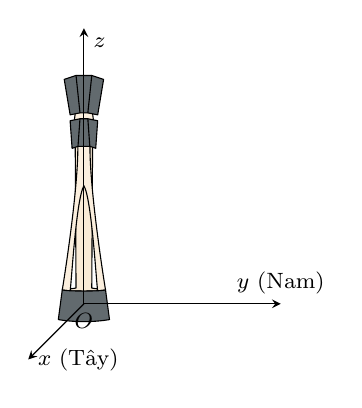
\begin{tikzpicture}[line join = round, line cap = round,>=stealth,font=\footnotesize,scale=1]
            \definecolor{antiquewhite}{rgb}{0.98, 0.92, 0.84}
            \definecolor{arsenic}{rgb}{0.23, 0.27, 0.29}
            \tikzset{tram/.pic={
                    \def\Tr{ 
                        (-.55,-1.65)
                        ..controls +(-10:.2) and +(-170:.2) ..(.55,-1.65)--(.2,-1.6)--(.22,2)--(-.22,2)--(-.2,-1.6)--cycle
                        
                        ;
                    }
                    \fill[antiquewhite] \Tr;
                    \draw[black]\Tr;
                    
                    \def\T{ 
                        (-.2,3)--(-.25,2.6)
                        ..controls +(-50:.5) and +(80:.2) ..(-.55,-1.65)--(-.35,-1.67)
                        ..controls +(80:.2) and +(-120:.4) ..(0,1)
                        ..controls +(-60:.4) and +(100:.2) ..(.35,-1.67)--(.55,-1.65)
                        ..controls +(100:.2) and +(-130:.5) ..(.25,2.6)--(.2,3)--cycle
                        ;
                    }
                    \fill[antiquewhite!80] \T;
                    \draw[black]\T;
                    
                    \def\A{ 
                        (-.5,3.7)--(-.35,2.8)--(-.1,2.85)--(.1,2.85)--(.35,2.8)--(.5,3.7)--(.2,3.8)--(-.2,3.8)--cycle
                        
                        (.1,2.7)--(-.1,2.7)--(-.35,2.65)--(-.3,1.95)--(-.15,2)--(.15,2)--(.3,1.95)--(.35,2.65)--(.1,2.7)
                        
                        (-.55,-1.65)
                        ..controls +(-10:.2) and +(-170:.2) ..(.55,-1.65)--(.65,-2.4)
                        ..controls +(-170:.4) and +(-10:.4) ..(-.65,-2.4)--cycle
                        ;
                    }
                    \fill[arsenic!80] \A;
                    \draw[black]\A;
                    \draw (.2,3.8)--(.1,2.85) (-.2,3.8)--(-.1,2.85)
                    (.1,2.7)--(.15,2) (-.1,2.7)--(-.15,2);
                    %===============================
                    \def\xmin{0} \def\xmax{3.5}
                    \def\ymin{-2} \def\ymax{5} 
                    \draw[->] (0,-2)--(5,-2) node [above]{$y$ (Nam)};
                    \draw[->] (0,\ymin)--(0,\ymax) node [below right]{$z$};
                    \draw[->] (0,-2)--++(-135:2) node [right]{$x$ (Tây)};
                    \draw (0,-2) node[below] {$O$};
                    
            }}
            
            \path (-2,-1)pic[scale=.5]{tram};
        \end{tikzpicture}
    }
    \choiceTF
    {Rađa ở vị trí có tọa độ $(0; 0; 0)$}
    {Vị trí $A$ có tọa độ $(350; 200; 12)$}
    {\True Khoảng cách từ máy bay đến rađa khoảng $403{,}29$ km (làm tròn kết quả đến hàng phần trăm)}
    {Nếu máy bay giữ nguyên độ cao, tiếp tục bay về phía nam $100$ km nữa thì rađa của trung tâm kiểm soát không lưu không phát hiện được vị trí của máy bay}
    \loigiai{
        \begin{center}
            \begin{tikzpicture}[line join = round, line cap=round,>=stealth,font=\footnotesize,scale=0.7]
                \path 
                (0,0) coordinate (O) 
                (5,0) coordinate (B)
                (-3,-2) coordinate (A)
                (0,4) coordinate (C)
                (4,5) coordinate (M)
                (2,0) coordinate (D1)
                (0,2) coordinate (E1)
                ($(E1)+(D1)-(O)$) coordinate (N1)
                ($(D1)+(M)-(N1)$) coordinate (P1)
                ($(P1)+(O)-(D1)$) coordinate (Q1)
                ($(E1)+(Q1)-(O)$) coordinate (K1)				
                ;
                \draw 	(O)--(B)(O)--(A) (O)--(C);
                
                \foreach \x/\r/\p in{A/180/x,B/90/y,C/90/z}
                \draw[->,line width=1pt] (O)--($(O)!1.2!(\x)$)node[scale=1.5,shift={(\r:3mm)}]{$\p$}; 
                ; 
                \draw[dashed] (D1)--(P1)--(Q1)--(O) (D1)--(N1)--(M)--(K1)--(E1)--(N1) (P1)--(M) (K1)--(Q1);
                \fill(D1)circle(1pt) (N1)circle(1pt) (E1)circle(1pt) (K1)circle(1pt) (Q1)circle(1pt) (P1)circle(1pt);	
                %\draw pic[draw,angle radius=7mm] {angle = M--O--C};
                \draw (D1) node[shift={(-90:5mm)}]{$200$};
                \draw (E1) node[shift={(180:4mm)}]{$12$};
                \draw (Q1) node[shift={(180:4mm)}]{$-350$};
                \draw (B) node[shift={(-70:4mm)}]{(Nam)};
                \draw (A) node[shift={(-30:4mm)}]{(Tây)};
                \draw (C) node[shift={(180:6mm)}]{(Trời)};			
                \draw (2,-2) node[shift={(-30:4mm)}]{(Mặt đất)};			
                %	\draw[dashed] (O)--(N)--(B) (A)--(N)--(M)--(C); 	
                \draw[->,line width=1pt] (O)--(M);				
                \draw (M) node[yshift=.4cm]{	
                    \begin{tikzpicture}[line join = round, line cap=round,>=stealth,font=\footnotesize,scale=0.15]						
                        \draw[cyan,line width=3pt] 
                        (0,0)--(0.2,-0.5)coordinate (A)--(5,-1.2)coordinate (O)
                        (10,0)--(9.8,-0.5)coordinate (A')--(5,-1.2)
                        (5,-0.8) circle(0.7cm) 
                        ($(A)!0.6!(O)+(0,-0.3)$) circle(0.3cm)
                        ($(A)!0.6!(O)+(0,-0.3)$) circle(0.2cm)		
                        ($(A')!0.6!(O)+(0,-0.3)$) circle(0.3cm)
                        ($(A')!0.6!(O)+(0,-0.3)$) circle(0.2cm)
                        (7,0)--(5,-0.3) -- (3,0)
                        (5,-0.3)--(5,1.2)
                        ;
                        \fill[cyan] (5,-0.8) circle(0.7cm);
                        
                        \fill[black,xshift=-0.05cm] (4.5,-0.7) rectangle (4.6,-0.5)
                        (4.7,-0.7) rectangle (4.8,-0.5)
                        (4.9,-0.7) rectangle (5,-0.5)
                        (5.1,-0.7) rectangle (5.2,-0.5)
                        (5.3,-0.7) rectangle (5.4,-0.5)
                        (5.5,-0.7) rectangle (5.6,-0.5)
                        ;			
                        \draw[line width=2pt] 
                        ($(A')!0.75!(O)$)--($(A')!0.75!(O)+(0,-0.65)$)
                        ($(A')!0.75!(O)+(0,-0.65)$)--++(0:0.2)
                        ($(A')!0.75!(O)+(0,-0.65)$)--++(180:0.2)--++(-90:0.1)
                        ($(A')!0.75!(O)+(0,-0.65)$)--++(180:0.2)--++(90:0.1)
                        ($(A')!0.75!(O)+(0,-0.65)$)--++(0:0.2)--++(-90:0.1)
                        ($(A')!0.75!(O)+(0,-0.65)$)--++(0:0.2)--++(90:0.1)
                        ($(A)!0.75!(O)$)--($(A)!0.75!(O)+(0,-0.65)$)
                        ($(A)!0.75!(O)+(0,-0.65)$)--++(0:0.2)
                        ($(A)!0.75!(O)+(0,-0.65)$)--++(180:0.2)--++(-90:0.1)
                        ($(A)!0.75!(O)+(0,-0.65)$)--++(180:0.2)--++(90:0.1)
                        ($(A)!0.75!(O)+(0,-0.65)$)--++(0:0.2)--++(-90:0.1)
                        ($(A)!0.75!(O)+(0,-0.65)$)--++(0:0.2)--++(90:0.1)
                        ;
                    \end{tikzpicture}	
                }
                ;
            \end{tikzpicture}
        \end{center}
        \begin{itemchoice}
            \itemch Rađa ở vị trí $B(0; 0; 0{,}1)$.
            \itemch Điểm $A(-350; 200; 12)$.
            \itemch Ta có $\overrightarrow{AB}=(350;-200;-11{,}9)$.\\
            Khoảng cách từ máy bay đến rađa là: $AB=\sqrt{350^2+200^2+11{,}9^2} \approx 403{,}29$ km.
            \itemch Nếu máy bay giữ nguyên độ cao, tiếp tục bay về phía nam $100$ km nữa thì máy bay đến vị trí điểm $C(-350; 300; 12)$. \\
            Ta có $\overrightarrow{BC}=(-350; 300;-11,9)$.\\
            Khoảng cách từ máy bay đến rađa là $BC=\sqrt{350^2+300^2+11{,}9^2} \approx 461{,}13$ km $< 500$ km.\\
            $\Rightarrow$ rađa của trung tâm kiểm soát không lưu vẫn phát hiện được vị trí của máy bay.
        \end{itemchoice}
    }
\end{ex}
\begin{ex}[MH-2025]
    \immini[thm]{
      Các thiên thạch có đường kính lớn hơn $140$ m và có thể lại gần Trái Đất ở khoảng cách nhỏ hơn $7\,500\,000$ km được coi là những vật thể có khả năng va chạm gây nguy hiểm cho Trái Đất. Để theo dõi những thiên thạch này, người ta đã thiết lập các trạm quan sát các vật thể bay gần Trái Đất. Giả sử có một hệ thống quan sát có khả năng theo dõi các vật thể ở độ cao không vượt quá $6\,600$ km so với mực nước biển. Coi Trái Đất là khối cầu có bán kính $6\,400$ km. Chọn hệ trục tọa độ $Oxyz$ trong không gian có gốc $O$ tại tâm Trái Đất và đơn vị độ dài trên mỗi trục tọa độ là $1\,000$ km. 
    }
    {
        \begin{tikzpicture}[line join = round, line cap=round,>=stealth,font=\footnotesize,transform shape,scale=0.8]
            \draw 
            (0,0) circle(3.5cm)
            ;
            \draw[fill=black!30] 
            (0,0) circle(1.6cm);
            \draw[<->] (0:3.5)--(0:1.6) node[pos=0.5,above]{$6\, 600$ km};
            \draw[<->] (0:0)--(0:1.6) node[pos=0.5,above]{$6\, 400$ km};
            \draw (130:3.5)coordinate (A)--(40:3.5)coordinate (B);
            \draw ($(A)!-0.4!(B)$) --(A)
            ($(A)!1.4!(B)$)--(B)
            ;
            
            \fill 
            (A)circle(1.5pt)node[above left]{$A$}
            (B)circle(1.5pt)node[above right]{$B$}
            ($(A)!-0.4!(B)$) circle(1.5pt)node[above]{$M$}
            ($(A)!1.4!(B)$)circle(1.5pt)node[above]{$N$}
            ;
            
        \end{tikzpicture}
    }
    Một thiên thạch (coi như một hạt) chuyển động với tốc độ không đổi theo một đường thẳng từ điểm $M(6;20;0)$ đến điểm $N(-6;-12;16)$.
    \choiceTF
    {\True Đường thẳng $MN$ có phương trình tham số là $\heva{&x = 6 + 3t \\& y = 20 + 8t \\& z = -4t}$, $(t \in \mathbb{R})$}
    {Vị trí đầu tiên thiên thạch đi chuyển vào phạm vi theo dõi của hệ thống quan sát là điểm $A(-3; -4; 12)$}
    {\True Khoảng cách giữa vị trí đầu tiên và vị trí cuối cùng mà thiên thạch di chuyển trong phạm vi theo dõi của hệ thống quan sát  là $18\,900$ km (kết quả làm tròn đến hàng trăm đơn vị ki-lô-mét)}
    {\True Nếu thời gian di chuyển của thiên thạch trong phạm vi theo dõi của hệ thống quan sát là $3$ phút thì thời gian nó di chuyển từ $M$ đến $N$ là $6$ phút}
    \loigiai{
        \begin{itemchoice}
            \itemch \textbf{Đúng}.\\
            Ta có $\overrightarrow{MN}=(-12;-32;16)=-4\cdot (3;8;-4)$.
            \\
            Suy ra $MN$ có một véctơ chỉ phương là $\overrightarrow{u}=(3;8;-4)$.
            \\
            Phương trình tham số của đường thẳng $MN$ là $\heva{&x = 6 + 3t \\& y = 20 + 8t \\& z = -4t}$, $(t \in \mathbb{R})$.
            
            \itemch \textbf{Sai.}\\
            \begin{center}
                \begin{tikzpicture}[line join = round, line cap=round,>=stealth,font=\footnotesize,transform shape,scale=0.7]
                    \draw 
                    (0,0)coordinate (O) circle(3.5cm)
                    ;
                    \draw[fill=black!30] 
                    (0,0) circle(1.6cm);
                    \draw[<->] (0:3.5)--(0:1.6) node[pos=0.5,above]{$6\, 600$ km};
                    \draw[<->] (0:0)--(0:1.6) node[pos=0.5,above]{$6\, 400$ km};
                    \draw (130:3.5)coordinate (A)--(40:3.5)coordinate (B);
                    \draw ($(A)!-0.4!(B)$) --(A)
                    ($(A)!1.4!(B)$)--(B)
                    ;
                    
                    \fill 
                    (A)circle(1.5pt)node[above left]{$A$}
                    (B)circle(1.5pt)node[above right]{$B$}
                    ($(A)!-0.4!(B)$)coordinate (M) circle(1.5pt) circle(1.5pt)node[above]{$M$}
                    ($(A)!1.4!(B)$) node[above]{$N$}
                    ;
                    \draw 
                    (O)--($(A)!1/2!(B)$)coordinate(H) 
                    (O)--(A)
                    (O)--(M)
                    ; 
                    
                    
                    \foreach \p/\r in {O/-90,H/90}
                    \fill (\p) circle (1.2pt) node[shift={(\r:3mm)}]{$\p$};			
                    
                    \draw pic[draw,angle radius=3mm] {right angle = O--H--A}; 
                    
                \end{tikzpicture}
            \end{center}
            Do $H\in MN\Rightarrow H(6+3t;20+8t;-4t)$ suy ra $\overrightarrow{OH}=(6+3t;20+8t;-4t)$ 
            \\
            Hơn nữa
            \begin{eqnarray*}
                OH\perp MN &\Leftrightarrow& \overrightarrow{OH}\cdot \overrightarrow{u}=0
                \\
                &\Leftrightarrow& 3(6 + 3t) + 8(20 + 8t) + (-4)\cdot (-4t)=0
                \\
                &\Leftrightarrow&178 + 89t=0 \Leftrightarrow t=-2.
            \end{eqnarray*}
            Suy ra $H(0;4;8)$ và độ dài của $OH=\sqrt{4^2+8^2}=4\sqrt 5$ (nghìn km).
            \\
            Xét tam giác $OMH$
            \\ 
            $OM=\sqrt{6^2+20^2+0}=2\sqrt{109}$ (nghìn km).
            \\
            Suy ra $MH=\sqrt{OM^2-OH^2}=\sqrt{436-80}=2\sqrt{89}$ (nghìn km).
            \\
            Xét tam giác $OAH$, ta có $OA=6\,400+6\,600=13$ (nghìn km).
            \\
            $AH=\sqrt{OA^2-OH^2}=\sqrt{169-80}=\sqrt{89}$ (nghìn km).
            \\
            Suy ra $MH=2AH$ hay $A$ là trung điểm $MH$.
            \\
            Vậy toạ độ $A(3;12;4)$.
            
            
            \itemch \textbf{Đúng.}
            \\
            Độ dài đoạn $AB=2AH=2\sqrt{89}\approx 18{,}87$ nghìn km tức là $AH=18\, 870$ km $\approx 18\, 900$ km.
            
            \itemch \textbf{Đúng.}
            \\
            Ta có $3$ phút bằng $\dfrac{1}{20}$ giờ và $3$ phút bằng $\dfrac{1}{10}$ giờ.
            \\
            Vận tốc của thiên thạch $v=\dfrac{AB}{\dfrac{1}{20}}=378\,000$ (km/h) $=378$ (nghìn km/h).
            \\
            Độ dài của $MN=2MH=4\sqrt{89}$ (nghìn km).
            \\
            Thời gian đi từ $M$ đến $N$ là $\dfrac{4\sqrt{89}}{378}\approx 0{,}1$ h bằng $6$ phút.
        \end{itemchoice}
    }
\end{ex}

\begin{ex}%[2H5V2-8]
\immini[thm]
{
        Trong không gian $Oxyz$, đơn vị trên mỗi trục tọa độ dài $1$ km, mặt đất là mặt phẳng $(Oxy$) một chiếc máy bay bắt đầu di chuyển từ điểm $A(700; 850; 100)$ với vận tốc không đổi $150$ km/h theo hướng về điểm $B(800; 900; 200)$. Khi tới $B$, máy bay thay đổi hướng bay theo hướng về điểm $C(1100; 1400; 300)$ với vận tốc giữ nguyên là $150$ km/h.
}
{
    \includegraphics[width=6cm]{images/maybay_DS}
}
Máy bay di chuyển theo hướng mới trong $30\sqrt{35}$ phút (tức là mới tới điểm $D \in BC$) thì bất ngờ gặp gió lớn, khiến hướng bay của nó lệch đi $45$ độ theo phương nằm ngang (tức là nếu $\vec{u}$ là vectơ hình chiếu xuống mặt đất của đoạn đường từ điểm $D$ trở đi thì góc lượng giác $(\vec{i}, \vec{u}) = 45^\circ$), và vận tốc giảm còn $120$ km/h. Máy bay tiếp tục bay theo hướng lệch trong $30$ phút. Xét tính đúng sai của các khẳng định sau:
    \choiceTF
    {Tổng thời gian bay thực tế của máy bay trong cả hành trình này là $142$ phút (kết quả làm tròn đến hàng đơn vị)} 
    {\True Khi bắt đầu gặp gió lớn, máy bay cách mặt đất $275$ km} 
    {Gọi $E(a; b; c)$ là vị trí cuối cùng của máy bay trong hành trình này, khi đó $a + b + c = 2670$ (làm tròn đến hàng đơn vị)} 
    {Tổng quãng đường cả hành trình dài hơn $650$ km} 
    \loigiai{Ta có $A(700, 850, 100)$, $B(800, 900, 200)$, $C(1100, 1400, 300)$.\\
        Ta có $\vec{AB} = (100, 50, 100)\Rightarrow |\vec{AB}| = \sqrt{100^2+50^2+100^2} = \sqrt{22500} = 150$ km.\\
        Ta có $\vec{BC} = (300, 500, 100)\Rightarrow |\vec{BC}| = \sqrt{300^2+500^2+100^2} = \sqrt{350000} = 100\sqrt{35}$.\\
        Thời gian bay  từ $A$ tới $B$ là $t_{AB} = \dfrac{|\vec{AB}|}{v_{AB}} = \dfrac{150}{150} = 1$ giờ $= 60$ phút.\\
        Thời gian từ $B$ tới $D$ là $t_{BD} =30\sqrt{30}$ phút.
        Thời gian từ $D$ tới $E$ là $t_{DE} =30$ phút.
        
        \begin{itemchoice}
            \itemch Sai. Tổng tời gian là $60+30\sqrt{35}+30\approx 267$ phút.
            \itemch Đúng.Ta có $\overrightarrow{v_{BD}}$ cùng hướng $\overrightarrow{B C}$ suy ra \\ $\overrightarrow{v}_{BD}=\left|\overrightarrow{v_{B D}}\right| \cdot \dfrac{\overrightarrow{BC}}{BC}=150\cdot \dfrac{(300, 500, 100)}{100\sqrt{35}}=150\cdot \dfrac{(3 ; 5 ; 1)}{\sqrt{35}}$.\\
            Ta có $\overrightarrow{B D}=t_{B \rightarrow D} \cdot \vec{v}_{B D}=\dfrac{\sqrt{35}}{2} \cdot \dfrac{150}{\sqrt{35}} \cdot(3 ; 5 ; 1)=(225 ; 375 ; 75)$.\\
            Mà  $B(800, 900, 200)$ nên $D(1025 ; 1275 ; 275)$.\\
            Vậy khi gặp gió máy bay cách mặt đất $275$ km.
            \itemch Sai. Gọi $\beta$ là góc tại bởi  $DE$ và mặt phẳng $(Oxy)$. \\
            Do máy bay chỉ đổi hướng và giữ nguyên tốc độ bay nên ta có \\
            $\beta=(DE,(Oxy))=(DC,(Oxy))=(BC,(Oxy))$.\\
            Khi đó $\sin \beta=\dfrac{|100|}{\sqrt{300^2+500^2+100^2}}=\dfrac{1}{\sqrt{35}}$. Suy ra $\cos \beta=\sqrt{\dfrac{34}{35}}$.\\
            Gọi $\overrightarrow{v'} $ là véc-tơ vận tốc khi máy bay đổi hướng.\\
            Khi đó ta có
            \begin{enumerate}[•]
                \item	$x_{\vec{v}'}=\left|\vec{v'}\right| \cdot \cos \beta \cdot \cos \alpha=120 \cdot \sqrt{\dfrac{34}{35}} \cdot \cos 45^{\circ}=\approx 83{,}63$.				
                \item 		$y_{\vec{v}'}=\left|\overrightarrow{u'}\right| \cdot \cos \beta \cdot \sin \alpha=120 \sqrt{\dfrac{34}{35}} \cdot \sin 45^{\circ} \approx 83{,}63$.						
                \item $z_{\overrightarrow{v}'}=\left|\vec{v}'\right| \cdot \sin \beta \quad=120 \cdot \dfrac{1}{\sqrt{35}} \approx 20{,}28$.
            \end{enumerate}	
            Ta lại có 	$\overrightarrow{DE}=t_{D \rightarrow E} \cdot \vec{v}'=\dfrac{1}{2} \cdot \overrightarrow{v}' \quad \Rightarrow \overrightarrow{OE}=\overrightarrow{OD}+\dfrac{1}{2} \overrightarrow{v}'$\\ mà  $D(1025 ; 1275 ; 275)$ nên 
            $\overrightarrow{DE}=D(1025 ; 1275 ; 275)+\dfrac{1}{2}\overrightarrow{v}'$.\\
            Suy ra $a+b+c=\left(1025+\dfrac{1}{2} \cdot 83{,}63\right)+\left(1275+\dfrac{1}{2} \cdot 83{,}63\right)+\left(275+\dfrac{1}{2} \cdot 20{,}28\right)\approx 2669$.
            \itemch Sai. Tổng quãng đường của cả hành trình\\
            $A B+B D+D E=150+75\sqrt{35}+120\cdot \dfrac{1}{2}\approx 653{,}7$.
        \end{itemchoice}		
    }
\end{ex}
\begin{ex}[SỞ BÌNH PHƯỚC]%[2H5V1-7]
    \immini[thm]{Một mái nhà hình tròn được đặt trên ba cây cột trụ. Các cây cột trụ vuông góc với mặt sàn nhà phẳng và có độ cao lần lượt là $8$ m, $9$ m, $10$ m. Ba chân cột là ba đỉnh của một tam giác đều trên mặt sàn nhà với cạnh dài $8$ m. Chọn hệ trục tọa độ như hình vẽ với $B \in Ox$, $C \in Oy$, tia $Oz$ cùng hướng với vectơ $\overrightarrow{AA'}$. Chọn gốc tọa độ $O$ trùng với trung điểm của $AC$ và mỗi đơn vị trên trục có độ dài $1$ m (xem hình vẽ).
    \choiceTF
    {\True Tọa độ các điểm $A'(0; -4; 10)$, $B'\left(4\sqrt{3}; 0; 9\right)$, $C'(0; 4; 8)$}
    {Mặt phẳng $(ABC)$ nhận $\overrightarrow{k}=(0; 1; 1)$ làm vectơ pháp tuyến}
    {\True Mặt phẳng $(A'B'C')$ nhận $\overrightarrow{n}=(0; 1; 4)$ làm vectơ pháp tuyến}
    {Biết độ dốc của mái nhà đạt mức tiêu chuẩn khoảng từ $27^\circ$ đến $35^\circ$ thì mái nhà trên có độ dốc ở mức tiêu chuẩn}
    }{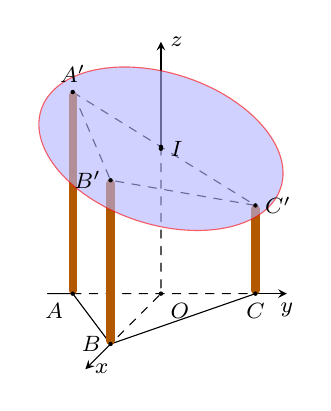
\begin{tikzpicture}[>=stealth,line join=round,line cap=round,font=\footnotesize,scale=0.8]
            \coordinate[] (I)at(0,2.3);	
            \coordinate[label=below right:$O$] (O)at(0,0);
            \draw[dashed,black]  (-1.4,3.2)coordinate(A')--(1.5,1.4)coordinate(C')--(-0.8,1.8)coordinate(B')--(A') (-1.4,0)coordinate(A)--(1.5,0)coordinate(C) (0,2.33)coordinate(T)--(O)--(-0.8,-0.8)coordinate(B);
            \draw (-1.8,0)--(A)--(B)--(C);
            \draw[->] (1.5,0)--(2,0)node[below]{$y$};
            \draw[->] (0,2.33)--(0,4)node[right]{$z$};
            \draw[->] (-0.8,-0.8)--(-1.2,-1.2)node[right]{$x$};
            \draw[line width=3pt,orange!70!black] (-1.4,0.05)--(-1.4,3.15) (1.5,0.05)--(1.5,1.35) (-0.8,-0.75)--(-0.8,1.75);
            \begin{scope}[rotate=-18]
                \draw[red,fill=blue!30,opacity=0.6] (I) ellipse (2cm and 1.2cm);
            \end{scope}	
            \foreach \diem in {T,O} \fill (\diem)circle(1pt);
            \foreach \diem/\vitri in {A/below left,B/left,C/below,A'/above,B'/left,C'/right,I/right} \fill (\diem)circle(1pt)node[\vitri]{$\diem$};
    \end{tikzpicture}}
    \loigiai{
        \begin{itemchoice}
            \itemch $A(0; -4; 0)$, $B\left(4\sqrt{3}; 0; 0\right)$, $C(0; 4; 0)$ và $A'(0; -4; 10)$, $B'\left(4\sqrt{3}; 0; 9\right)$, $C'(0; 4; 8)$.
            \itemch Vectơ pháp tuyến của mặt phẳng $(ABC)$ là $\vec{k}(0; 0; 1)$.
            \itemch $\overrightarrow{A'B'} = \left(4\sqrt{3}; 4; -1\right)$, $\overrightarrow{A'C'} = (0; 8; -2)$, khi đó vectơ pháp tuyến của $(A'B'C')$ là \[\left[\overrightarrow{A'B'}, \overrightarrow{A'C'}\right] = 8\sqrt{3}(0; 1; 4).\]
            \itemch Vectơ pháp tuyến của mặt phẳng $(ABC)$ là $\overrightarrow{k}=(0; 0; 1)$.\\
            Khi đó $\cos\left((ABC), (A'B'C')\right) = \dfrac{4\sqrt{17}}{17}$ nên $\left((ABC), (A'B'C')\right) \approx 14^\circ$ nên mái nhà không ở mức tiêu chuẩn.
        \end{itemchoice}
    }
\end{ex}

\begin{ex}%[Dự án C THPTQG 2025]%[Võ Hoàng Nghĩa]%[2H5V2-7]
    \immini{Trong không gian $Oxyz$, một cabin cáp treo xuất phát từ điểm $A(10;3;0)$ và chuyển động đều theo đường cáp có vectơ chỉ phương $\vec{u}=(2;-2;1)$ (hướng chuyển động cùng chiều với hướng vectơ $\vec{u}$ với tốc độ là $4{,}5$ (m/s); đơn vị trên mỗi trục là mét).}{	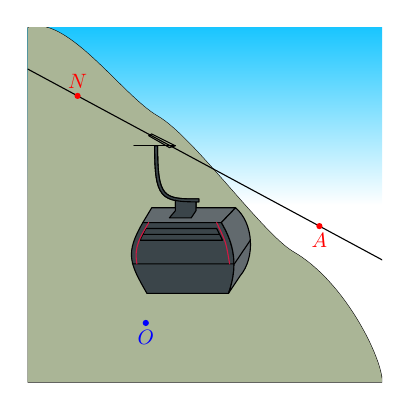
\begin{tikzpicture}[line join=round,line cap=round,scale=0.75,transform shape]%cau18
            \definecolor{ecru}{rgb}{0.76,0.7,0.5} 
            \definecolor{darkolivegreen}{rgb}{0.33,0.42,0.18} 
            \definecolor{deepskyblue}{rgb}{0.0,0.75,1.0} 
            \definecolor{antiquebrass}{rgb}{0.8,0.58,0.46}
            \definecolor{arsenic}{rgb}{0.23,0.27,0.29} 
            \definecolor{ashgrey}{rgb}{0.7,0.75,0.71}\definecolor{alizarin}{rgb}{0.82,0.1,0.26} 
            \clip (-3,-3) rectangle (3,3);
            \fill[bottom color=white,top color=deepskyblue!90,middle color=white] (-3,-3) rectangle (3,3);
            \tikzset{dat/.pic={
                    \def\N{
                        (-3,3) 
                        ..controls +(20:.7) and +(150:.7)..(-.8,1.5) 
                        ..controls +(-30:.7) and +(150:.6)..(1.5,-.8)
                        ..controls +(-30:1) and +(90:.4)..(3,-3)--(-3,-3)--cycle;
                    } 
                    \draw[black]\N; 
                    \fill[darkolivegreen!50] \N;
            }}
            \tikzset{cap_treo/.pic={
                    \def\X{
                        (-.85,1)--(-.8,1)
                        ..controls +(-90:.9) and +(-180:.6)..(-.1,0.1)--(-.1,.05)
                        ..controls +(-180:.65) and +(-90:.9)..cycle
                        (-.15,0.05)--(-.15,-.1)--(-.23,-.22)--(-.6,-.22)--(-.5,-.1)--(-.5,.08); 
                    } 
                    %\fill[black] \X;
                    \draw\X; 
                    \draw (-3,2.3)--(3.5,-1.2); 
                    \draw (-1.2,1)--(-.5,1);
                    \draw (-.5,1)--(-.9,1.2)--(-.95,1.17)--(-.6,.97)--cycle;
                    \draw[fill=arsenic!80](-.9,-.05)--(.52,-.05)--(.28,-.3)--(-1.05,-.3)--cycle;
                    \def\M{ 
                        (-.85,1)--(-.8,1)
                        ..controls +(-90:.9) and +(-180:.6)..(-.1,0.1)--(-.1,.05)
                        ..controls +(-180:.65) and +(-90:.9)..cycle
                        (-.15,0.05)--(-.15,-.1)--(-.23,-.22)--(-.6,-.22)--(-.5,-.1)--(-.5,.08);
                    } 
                    \fill[arsenic] \M;
                    \draw\M;
                    \def\N{
                        (-1.05,-.3) 
                        ..controls +(-120:.6) and +(120:.6)..(-.98,-1.5)--(.4,-1.5)
                        ..controls +(70:.6) and +(-60:.3)..(.28,-.3)--cycle;
                    }
                    \fill[arsenic] \N; 
                    \draw\N; 
                    \def\P{ 
                        (.4,-1.5)
                        ..controls +(70:.6) and +(-60:.3)..(.28,-.3)--(.52,-.05)
                        ..controls +(-40:.4) and +(50:.4)..(.6,-1.2)--cycle;
                    }
                    \fill[arsenic!80] \P;
                    \draw\P; 
                    \draw (-1.23,-1)--(.5,-1)--(.77,-.6);
                    \draw (-1.05,-.5)--(-1,-.4)--(.2,-.4)--(.25,-.5)--cycle
                    (.25,-.5)--(.3,-.6)--(.3,-.6)--(-1.1,-.6)--(.-1.05,-.5)--cycle; 
                    \draw[alizarin](.42,-1)..controls +(100:.4) and +(-65:.4)..(.2,-.3); 
                    \draw[alizarin](-1.15,-1)..controls +(100:.3) and +(-120:.3)..(-.95,-.3); 
            }}
            \path 
            (0,0) pic[scale=1]{dat}
            (0,0) pic[scale=1]{cap_treo};
            \path (-3,2.3)--(3.5,-1.2)
            coordinate[pos=0.13](N)
            coordinate[pos=0.76](A);
            \fill[red] (N) circle (1.5pt) node[above]{$N$};
            \fill[red] (A) circle (1.5pt) node[below]{$A$};
            \fill[blue] (-1,-2) circle (1.5pt) node[below]{$O$};
    \end{tikzpicture}}
    \choiceTF
    {\True Phương trình tham số của đường cáp là $\heva{&x=10+2k\\&y=3-2k\\&z=k,}(k\in\mathbb{R})$}
    {\True Giả sử sau thời gian $t$ (s) kể từ khi xuất phát ($t\geq 0$), cabin đến điểm $M$. Khi đó tọa độ điểm $M$ là $\left(3t+10;-3t+3;\dfrac{3t}{2}\right)$}
    {Cabin dừng ở điểm $B$ có hoành độ $x_B=550$, khi đó quãng đường $AB$ dài $800$ m}
    {Đường cáp $AB$ tạo với mặt phẳng $(Oxy)$ một góc $30^\circ$}
    \loigiai{
        \begin{itemchoice}
            \itemch Phương trình tham số của đường thẳng $d$ qua $A(10;3;0)$ và có VTCP $\overrightarrow{u}=(2 ;-2 ; 1)$ là $\heva{&x=10+2k\\&y=3-2k\\&z=k}(k\in\mathbb{R}).$
            \itemch Ta có độ dài $AM=v\cdot t = 4{,}5t$.\\
            Vì $M$ thuộc đường thẳng $d$ nên $M$ có tọa độ $(10+2k; 3-2k;k), (k\in\mathbb{R})$.\\
            Vì $\vec{AM}=(2k;-2k;k)$ mà $\vec{AM}$ cùng hướng với $\vec{u}$ nên có $k \geq 0$, hay $AM=3k$.\\
            Suy ra $3k=4{,}5t \Rightarrow k=1{,}5t$ do đó tọa độ điểm $M$ là $\left(3t+10;-3t+3; \dfrac{3t}{2}\right)$.
            \itemch Ta thấy khi $x_B=550$ tức tà $3t+10=550$ thì $t=180$ (s).\\
            Vậy $AB=v\cdot t=4{,}5\cdot 180=810$ (m).
            \itemch Ta có $\overrightarrow{u_{AB}}=(2;-2;1)$. Ngoài ra, mặt phẳng ($Oxy$) có phương trình $z=0$ nên có một vectơ pháp tuyến $\overrightarrow{n}=(0;0;1)$.\\
            Gọi $\alpha$ là góc giữa $AB$ và ($Oxy$), ta có $\sin \alpha=\dfrac{|\overrightarrow{u}\cdot \vec{n}|}{|\overrightarrow{u}|\cdot|\overrightarrow{n}|}=\dfrac{1}{3}$.\\
            Suy ra $\alpha\approx 19{,}47^\circ$.
        \end{itemchoice}
    }
\end{ex}


\begin{ex}[MH-2025]
    Hệ thống định vị toàn cầu GPS là một hệ thống cho phép xác định vị trí của một vật thể trong không gian. Trong cùng một thời điểm, vị trí của một điểm $M$ trong không gian sẽ được xác định bởi bốn vệ tinh cho trước nhờ các bộ thu phát tín hiệu đặt trên các vệ tinh. Giả sử trong không gian với hệ tọa độ $Oxyz$, có bốn vệ tinh lần lượt đặt tại các điểm $A(3;1;0)$, $B(3;6;6)$, $C(4;6;2)$, $D(6;2;14)$; vị trí $M(a;b;c)$ thỏa mãn $MA = 3$, $MB = 6$, $MC = 5$, $MD = 13$. Khoảng cách từ điểm $M$ đến điểm $O$ bằng bao nhiêu?
    \shortans{3}
    \loigiai{
        Giả sử $M(a;b;c)$. Ta có
        \begin{eqnarray*}
            MA=3&\Leftrightarrow& \sqrt{(a-3)^2+(b-1)^2+c^2}=3
            \\
            MB=6&\Leftrightarrow&\sqrt{(a-3)^2+(b-6)^2+(c-6)^2}=6
            \\
            MC=5&\Leftrightarrow&\sqrt{(a-4)^3+(b-6)^2+(c-2)^2}=5
            \\
            MD=13&\Leftrightarrow&\sqrt{(a-6)^3+(b-2)^2+(c-14)^2}=13
        \end{eqnarray*}
        Ta có hệ phương trình $\heva{
            & a^2 + b^2 + c^2 - 6a - 2b + 1 = 0\\
            & a^2 + b^2 + c^2 - 6a - 12b - 12c + 45 = 0 \\
            & a^2 + b^2 + c^2 - 8a - 12b - 4c + 31 = 0 \\
            & a^2 + b^2 + c^2 - 12a - 4b - 28c + 67 = 0.
        }$
        \\
        Giữ nguyên phương trình thứ nhất, lấy phương trình thứ nhất trừ vế theo vế với các phương trình còn lại ta được hệ phương trình mới như sau 
        \\
        $\heva{
            & a^2 + b^2 + c^2 - 6a - 2b + 1 = 0 \\
            & 10b + 12c = 44 \\
            & 2a + 10b + 4c = 30 \\
            & 6a + 2b + 28c = 66
        }\Leftrightarrow \heva{
            & a^2 + b^2 + c^2 - 6a - 2b + 1 = 0 \\
            & a = 1 \\
            & b = 2 \\
            & c = 2.
        }$
        \\
        Thế $a=1$, $b=2$, $c=2$ vào phương trình thứ nhất ta thấy thoả mãn. 
        \\
        Vậy điểm $M(1;2;2)\Rightarrow OM=\sqrt{1+4+4}=3$.
    }
\end{ex}
\begin{ex}%[2H5V3-4]%[ĐỀ ÔN THI TỐT NGHIỆP 2025 - SỐ 2- Hector Tran]%[THPT Lê Quý Đôn- Tỉnh Đồng Nai]
    Trong không gian $Oxyz$, cho mặt cầu $(S)\colon x^2+y^2+z^2+2x-4y-2z+\dfrac{9}{2}=0$ và hai điểm $A(0;2;0)$, $B(2;-6;-2)$. Điểm $M(a;b;c)$ thuộc $(S)$ thỏa mãn $\overrightarrow{MA}\cdot\overrightarrow{MB}$ có giá trị nhỏ nhất. Tổng $a+b+c$ bằng bao nhiêu?
    \shortans{1}
    \loigiai{
        Ta có $(S)\colon x^2+y^2+z^2+2x-4y-2z+\dfrac{9}{2}=0\Leftrightarrow (S)\colon (x+1)^2+(y-2)^2+(z-1)^2=\dfrac{3}{2}$.\\
        Mặt cầu $(S)$ có tâm $I(-1;2;1)$, bán kính $R=\dfrac{\sqrt{6}}{2}$.\\
        Vì $IA=\sqrt{2}>R$ và $IB=\sqrt{82}>R$ nên hai điểm $A$, $B$ nằm ngoài mặt cầu $(S)$.\\
        Gọi $K$ là trung điểm đoạn thẳng $AB$ thì $K(1;-2;-1)$ và $K$ nằm ngoài mặt cầu $(S)$.\\
        Ta có \begin{eqnarray*}
            \overrightarrow{MA}\cdot\overrightarrow{MB}&=&\left(\overrightarrow{MK}+\overrightarrow{KA}\right)\cdot\left(\overrightarrow{MK}+\overrightarrow{KB}\right)\\
            &=&MK^2+\overrightarrow{MK}\cdot \left(\overrightarrow{KA}+\overrightarrow{KB}\right)+\overrightarrow{KA}\cdot\overrightarrow{KB}\\
            &=&MK^2-KA^2.
        \end{eqnarray*}		
        Suy ra $\overrightarrow{MA}\cdot\overrightarrow{MB}$ nhỏ nhất khi $MK^2$ nhỏ nhất, tức là $MK$ nhỏ nhất.\\
        Đánh giá $IM+MK\ge IK\Rightarrow R+MK\ge IK\Rightarrow MK$ $\ge IK-R$.\\
        Suy ra $MK$ nhỏ nhất bằng $IK-R$, xảy ra khi $I$, $M$, $K$ thẳng hàng và $M$ nằm giữa hai điểm $I$, $K$.\\
        Như vậy $M$ là giao điểm của đoạn thẳng $IK$ và mặt cầu $(S)$.\\
        Ta có $\overrightarrow{IK}=(2;-4;-2)$, $IK=\sqrt{2^2+(-4)^2+(-2)^2}=2\sqrt{6}=4R=4IM$.\\
        Suy ra $\overrightarrow{IK}=4\overrightarrow{IM}\Leftrightarrow \heva{&2=4(a+1)\\&-4=4(b-2) \\&-2=4(c-1)}\Leftrightarrow \heva{&a=-\dfrac{1}{2}\\&b=1\\&c=\dfrac{1}{2}.}$\\
        Vậy $a+b+c=1$.		
    }
    \dotlineEX{2}
\end{ex}
\begin{ex}[KHTN-HÀ NỘI - LẦN 2]%[2H5V2-7]
    Trong không gian  $Oxyz$, cho điểm $M(2;1;1)$ và đường thẳng $d\colon \dfrac{x-3}{1} = \dfrac{y-3}{-1} = \dfrac{z+1}{-2}$.
    Đường thẳng $\Delta$ đi qua điểm $M$, song song với mặt phẳng $(Q)\colon x-2y+z-3 = 0$ và tạo với $d$ góc nhỏ nhất. Gọi $A(-8; h; k)$ là một điểm nằm trên $\Delta$. Tính giá trị $h+k$.
    \shortans{$36$}
    \loigiai{
        Giả sử đường thẳng $\Delta$ có một éc-tơ chỉ phương $\overrightarrow{u} = (a;b;c) \neq \overrightarrow{0}$.\\
        Đường thẳng $d$ có một éc-tơ chỉ phương $\overrightarrow{u}_d = (1;-1;-2)$, mặt phẳng $(Q)$ có một éc-tơ pháp
        tuyến $\overrightarrow{n} = (1;-2;1)$.\\ 
        Vì $\Delta \parallel (Q)$, nên $\overrightarrow{u} \perp \overrightarrow{n} \Leftrightarrow \overrightarrow{u}\cdot\overrightarrow{n} = 0 \Leftrightarrow a - 2b + c = 0 \Leftrightarrow c = -a + 2b$.\\
        Khi đó $\overrightarrow{u} = (a;b;-a+2b)$, ta có $(\widehat{d,\Delta})$ bé nhất khi $\cos{(\widehat{d,\Delta})}$ lớn nhất.
        \begin{eqnarray*}
            \cos(\widehat{d, \Delta}) &=& \dfrac{|\overrightarrow{u}_d.\overrightarrow{u}|}{|\overrightarrow{u}_d|.|\overrightarrow{u}|}\\
            &=& \dfrac{|a-b-2(-a+2b)|}{\sqrt{1^2+(-1)^2+(-2)^2}.\sqrt{a^2+b^2+(-a+2b)^2}} \\
            &=& \dfrac{|3a-5b|}{\sqrt{6}.\sqrt{2a^2-4ab+5b^2}}\\
            &=& \dfrac{1}{\sqrt{6}}\sqrt{\dfrac{9a^2-30ab+25b^2}{2a^2-4ab+5b^2}}.
        \end{eqnarray*}
        Xét $b = 0 \Rightarrow \cos(d, \Delta) = \dfrac{\sqrt{3}}{2} \Rightarrow (d, \Delta) = 30^\circ$.\\
        Xét $b \neq 0$, chia tử và mẫu của phân thức dưới dấu căn cho $b^2$ và đặt $t = \dfrac{a}{b}$, ta được
        $$\cos(a, \Delta) = \dfrac{1}{\sqrt{6}} \sqrt{\dfrac{9t^2 - 30t + 25}{2t^2 - 4t + 5}}.$$
        Xét hàm $f(t) = \dfrac{9t^2 - 30t + 25}{2t^2 - 4t + 5}$, ta có\\
        $f'(t) = \dfrac{24t^2 - 10t - 50}{(2t^2 - 4t + 5)^2} \Rightarrow f'(t) = 0 \Leftrightarrow 24t^2 - 10t - 50 = 0 \Leftrightarrow \hoac{& t = \dfrac{5}{3} \\ & t = -\dfrac{5}{4}}$.\\
        Bảng biến thiên
        \begin{center}
            
\begin{tikzpicture}[scale=1, font=\footnotesize, line join=round, line cap=round, >=stealth]
                \tkzTabInit[nocadre,lgt=1,espcl=2,deltacl=0.5]
                {$t$/.7 ,$f'$/.7,$f$/2}
                {$-\infty$ , $-\dfrac{5}{4}$ , $\dfrac{5}{3}$ , $+\infty$}
                \tkzTabLine{ , + , $0$ , - , $0$ , + , }
                \tkzTabVar{-/$\dfrac{9}{2}$ , +/$\dfrac{35}{6}$ , -/$0$ , +/$\dfrac{9}{2}$}
            \end{tikzpicture}
        \end{center}
        Khi đó $\max f(t) = \dfrac{35}{6}$ khi $t = -\dfrac{5}{4} \Rightarrow \max \cos (d, \Delta) = \dfrac{\sqrt{35}}{6}$ khi $t = -\dfrac{5}{4}$ hay $\dfrac{a}{b} = -\dfrac{5}{4}$.\\
        Chọn $a = -5$, $b = 4$. Khi đó đường thẳng $\Delta$ đi qua điểm $M(2;1;1)$ và có một éc-tơ chỉ phương $\overrightarrow{u} = (-5; 4; 13)$, nên có phương trình $\Delta\colon \dfrac{x - 2}{-5} = \dfrac{y - 1}{4} = \dfrac{z - 1}{13}$.\\
        Vì $A(-8; h; k) \in \Delta \Rightarrow \dfrac{-8 - 2}{-5} = \dfrac{h - 1}{4} = \dfrac{b - k}{13} \Rightarrow \heva{&h = 9 \\& k = 27. }$\\
        Do đó $h + k = 36$.
    }
    \dotlineEX{2}
\end{ex}
\begin{ex}[CHUYÊN PHAN BỘI CHÂU - HÀ TĨNH]%[2H5V2-8]
    Người ta thiết kế một dây cáp chạy thẳng từ điểm $X$ ở trên mặt đất tới đỉnh $T$ của một tòa tháp. Giả sử tọa độ của các điểm là $T(40;60;150)$ và $X(100;-40;0)$ trong hệ tọa độ không gian $Oxyz$, với $O$ là gốc tọa độ đặt tại mặt đất. Người ta muốn nối điểm $A(40;30;-20)$ nằm dưới một cái hồ tới một điểm $M(a;b;c)$ nằm trên dây cáp  sao cho khoảng cách $MA$ này là nhỏ nhất. Tính $a+b+c$.
    \shortans{$100$}
    \loigiai
    {
        Ta có phương trình đường thẳng $(TX)\colon\heva{&x = 100 + 6t\\&y = -40 - 10t\\&z = -15t.}$\\
        $M(a; b; c)$ nằm trên dây cáp nên $M(100 + 6t; -40 - 10t; -15t)$.\\
        Khoảng cách $MA$ này là nhỏ nhất khi $\vv{MA}$ vuông góc với đường thẳng $(TX)$.\\
        Khi đó ta có $\vv{AM} \cdot \vv{TX} = 0 \Leftrightarrow t = \dfrac{-40}{19} \Rightarrow M\left( \dfrac{1660}{19};\ \dfrac{-360}{19};\ \dfrac{600}{19} \right)$.\\
        Vậy $a + b + c = 100$.
    }
    \dotlineEX{1}
\end{ex}

\begin{ex}%[2H5V1-3]
    \immini[thm]{Trong không gian $Oxyz$, cho bốn điểm $S$, $A$, $B$, $C$ như hình bên (mỗi ô lưới là $1$ đơn vị). Xét hình nón $(N)$ có đỉnh $S$, điểm $A$ thuộc đường sinh và hai điểm $B$, $C$ thuộc đường tròn đáy. Biết rằng, mặt phẳng $(P)$ chứa đường tròn đáy của $(N)$ đi qua điểm $D(x;1;1)$. Tính giá trị của $x$.
        \shortans{$7$}}
    {
        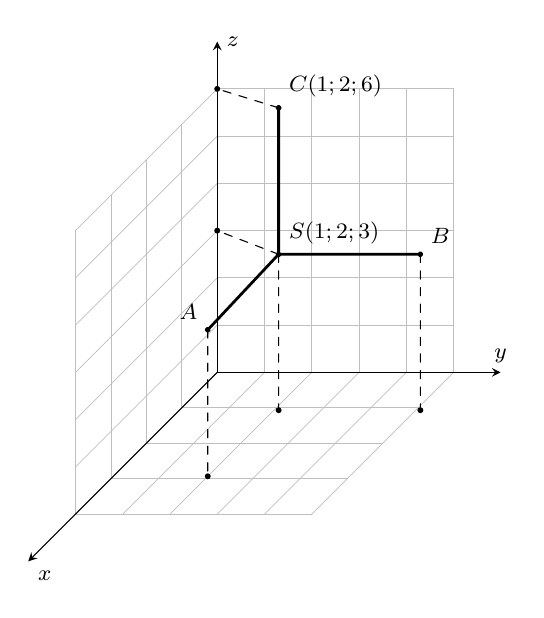
\begin{tikzpicture}[font=\footnotesize, line join=round, line cap=round, >=stealth, scale=0.6]
            \path (0,0)--(-3,-3)foreach \i in{0,1,2,...,4}{coordinate[pos=\i/4](A\i)};
            \path (5,0)--(2,-3)foreach \i in{0,1,2,...,4}{coordinate[pos=\i/4](A'\i)};
            \path (0,0)--(5,0)foreach \i in{0,1,2,...,5}{coordinate[pos=\i/5](B\i)};
            \path (-3,-3)--(2,-3)foreach \i in{0,1,2,...,5}{coordinate[pos=\i/5](B'\i)};
            \path (5,0)--(5,6)foreach \i in{0,1,2,...,6}{coordinate[pos=\i/6](B''\i)};
            \path (0,0)--(0,6)foreach \i in{0,1,2,...,6}{coordinate[pos=\i/6](C\i)};
            \path (0,6)--(5,6)foreach \i in{0,1,2,...,5}{coordinate[pos=\i/5](D\i)};
            \path (-3,-3)--(-3,3)foreach \i in{0,1,2,...,6}{coordinate[pos=\i/6](C'\i)};
            \path (0,6)--(-3,3)foreach \i in{0,1,2,...,4}{coordinate[pos=\i/4](D'\i)};
            \foreach \i in{0,1,2,...,4}
            \draw[gray!50,line width=.1mm] (A\i)--(A'\i);
            \foreach \i in{0,1,2,...,5}
            \draw[gray!50,line width=.1mm] (B\i)--(B'\i);
            \foreach \i in{0,1,2,...,6}
            \draw[gray!50,line width=.1mm] (B''\i)--(C\i);
            \foreach \i in{0,1,2,...,5}
            \draw[gray!50,line width=.1mm] (B\i)--(D\i);
            \foreach \i in{0,1,2,...,6}
            \draw[gray!50,line width=.1mm] (C'\i)--(C\i);
            \foreach \i in{0,1,2,...,4}
            \draw[gray!50,line width=.1mm] (A\i)--(D'\i);
            \draw[->] (0,0)--(-4,-4)node[below right]{$x$};
            \draw[->] (0,0)--(6,0)node[above] {$y$};
            \draw[->] (0,0)--(0,7)node[right] {$z$};
            \draw[line width=1](-0.2,0.9)circle(1pt)node[above left]{$A$}-- (1.3,2.5)--(4.3,2.5)circle(1pt)node[above right]{$B$}(1.3,2.5)circle(1pt)node[above right]{$S(1;2;3)$}--(1.3,5.6)circle(1pt)node[above right]{$C(1;2;6)$};
            \draw[dashed](-0.2,0.9)--(-0.2,-2.2) (1.3,2.5)--(1.3,-0.8)(4.3,2.5)--(4.3,-0.8)(1.3,2.5)--(0,3)(1.3,5.6)--(0,6);
            \fill (1.3,-0.8)circle(1.8pt)
            (4.3,-0.8)circle(1.8pt)
            (0,3)circle(1.8pt)
            (0,6)circle(1.8pt)
            (-0.2,-2.2)circle(1.8pt);
        \end{tikzpicture}
    }
%    \loigiai{
%        \immini{Dựa vào hình vẽ ta có $A(3;2;3)$ và $B(1;5;3)$.\\
%            Ta có $\overrightarrow{SC}=(0;0;3)\Rightarrow SC=3$;\\ $\overrightarrow{SA}=(2;0;0)\Rightarrow SA=2$.\\
%            Gọi $I$ là giao điểm của $SA$ và đường tròn đáy của hình nón.\\
%            Khi đó $SI=SC=3$.\\
%            Suy ra $SI=\dfrac{3}{2}\overrightarrow{SA}=(3;0;0)\Rightarrow I(4;2;3)$.\\
%            Khi đó mặt phẳng $(P)$ chứa đường tròn đáy của $(N)$ là mặt phẳng $(BCI)$.\\
%            Ta tìm được $(BCI):x+y+z-9=0$.\\
%            Vì $D(x;1;1)\in(BCI)$ nên $x+1+1-9=0\Leftrightarrow x=7$.}
%        {
%            \begin{tikzpicture}[font=\footnotesize, line join=round, line cap=round, >=stealth, scale=0.85]
%                \def \h{6}
%                \path (0,0) coordinate (O)
%                (180:3) coordinate (M)
%                (0:3) coordinate (I)
%                ($(O)+(0,\h)$) coordinate (S)
%                (M) arc(180:140:3 and 1) coordinate (C)
%                (M) arc(180:280:3 and 1) coordinate (B)
%                ($(S)!0.6!(I)$) coordinate (A)
%                ;
%                \draw[dashed] (M) arc(180:0:3 and 1) (C)--(I)--(B)--cycle (S)--(O);
%                \draw (M) arc(180:360:3 and 1)--(I)--(S)--(M) (S)--(B)(S)--(I);
%                \draw (C)circle(1pt)node[below]{$C$} (B)circle(1pt)node[below]{$B$} (I)circle(1pt)node[right]{$I$} (A)circle(1pt)node[right]{$A$} (S)circle(1pt)node[above]{$S$}(O)circle(1pt)node[below]{$O$};
%            \end{tikzpicture}
%        }
%    }
\dotlineEX{2}
\end{ex}
\begin{ex}%[2H2V2-6]
    Trong không gian $Oxyz$, đài kiểm soát không lưu sân bay đặt tại điểm có toạ độ $O(0; 0; 0)$, đơn vị trên mỗi trục tính theo kilômét. Một máy bay chuyển động hướng về đài kiểm soát không lưu, bay qua hai vị trí $A(-500;-250; 150)$, $B(-200;-200;100)$. Khi máy bay ở gần đài kiểm soát nhất, vị trí của máy bay ở điểm có tọa độ là $(a; b; c)$. Giá trị của biểu thức $T=-3a-b-c$ bằng bao nhiêu (làm tròn kết quả đến hàng đơn vị)?
    \shortans[]{$-11$}
    \loigiai{
        Vectơ $\vec{AB} = (300; 50; -50)$ nên $\vec{u} = (6; 1; -1)$ là một vectơ chỉ phương của đường thẳng $AB$.\\		
        Phương trình đường thẳng $AB$ là
        \[
        \begin{cases}
            x = -500 + 6t \\ 
            y = -250 + t \\ 
            z = 150 - t.
        \end{cases}
        \]		
        Gọi $H$ là hình chiếu của điểm $O$ trên đường thẳng $AB$ thì $OH$ là khoảng cách ngắn nhất giữa máy bay và đài kiểm soát. Khi đó, 
        \[
        H(6t - 500; t - 250; -t + 150).
        \]		
        Ta có
        \[
        \overrightarrow{OH} \cdot \vec{u} = (6t - 500) \cdot 6 + t - 250 + (-t + 150) \cdot (-1) = 0
        \]
        \[
        \Leftrightarrow t = \dfrac{1700}{19}.
        \]		
        Suy ra tọa độ vị trí máy bay khi đó là
        \[
        \left( \dfrac{700}{19}; \dfrac{-3050}{19}; \dfrac{1150}{19} \right).
        \]		
        Vậy $T = -3a - b - c = -\dfrac{200}{19} \approx -11$.
    }
    \dotlineEX{1}
\end{ex}
\begin{ex}%[2H2V2-6]%[THPT Văn Giang Hưng Yên-L3-2425-ChuHa]
    \immini[thm]
    {
        Với hệ trục tọa độ $Oxyz$ sao cho $O$ nằm trên mặt nước, mặt phẳng $Oxy$ là mặt nước, trục $Oz$ hướng lên trên (đơn vị đo: mét), một con chim bói cá đang ở vị trí cách mặt nước $2$ m, cách mặt phẳng $(Oxz)$, $(Oyz)$ lần lượt là $3$ m và $1$ m phóng thẳng xuống vị trí con cá, biết con cá cách mặt nước $50$ cm, cách mặt phẳng $(Oxz)$, $(Oyz)$ lần lượt là $1$ m và $1{,}5$ m. Tọa độ điểm $B$ lúc chim bói cá vừa tiếp xúc với mặt nước là $(a, b, c)$. Giá trị của $T = 5a + 15b + 25c$ bằng?
       \shortans[0]{28}
    }
    {
        \begin{tikzpicture}[line join=round, line cap=round,scale=1,transform shape, >=stealth]
            \definecolor{columbiablue}{rgb}{0.61, 0.87, 1.0}%màu nước
            \definecolor{arsenic}{rgb}{0.23, 0.27, 0.29}%màu mỏ
            \definecolor{antiquewhite}{rgb}{0.98, 0.92, 0.84}%màu trắng
            \definecolor{cadmiumorange}{rgb}{0.93, 0.53, 0.18}%lông cam
            \definecolor{coolblack}{rgb}{0.0, 0.18, 0.39}%cánh đậm
            \definecolor{brandeisblue}{rgb}{0.0, 0.44, 1.0}%màu xanh đầu
            \definecolor{darkcoral}{rgb}{0.8, 0.36, 0.27}%màu chân
            
            %---------màu vẽ cá
            \definecolor{amber}{rgb}{1.0, 0.49, 0.0}
            % \clip (-3,-3.5) rectangle (3.5,3);
            
            \tikzset{san/.pic={ 
                    \path
                    (-1.3,-1.5) coordinate (O)
                    ($(O)+(-142:2)$) coordinate (y)
                    ($(O)+(0:4.7)$) coordinate (x)
                    ($(O)+(90:3)$) coordinate (z)
                    ($(x)+(y)-(O)$) coordinate (t)					
                    (-.8,-2.2)coordinate (A)
                    (1.6,0.8) coordinate (C)
                    ($(A)!.13!(C)$) coordinate (B)
                    ;
                    \fill[columbiablue] (O)--(x)--(t)--(y)--cycle;
                    
                    \foreach\p/\g/\t in {x/110/y, y/150/x, z/-30/z}
                    {
                        \node at (\p) [shift=(\g:2mm)] {$\t$};
                    }					
                    \foreach \x/\pos in {A/170,B/0,C/-60,O/150} \fill (\x) circle(1pt) node[{shift=(\pos:0.25)}]{$\x$}; 
                    
                    \draw[->] (O)--(x) ;
                    \draw[->] (O)--(y);
                    \draw[->] (O)--(z);
                    \draw[dashed] (A)--(B);
                    \draw (B)--(C);
                    %---------nước
                    \draw (-1,-1.7)
                    ..controls +(-120:.5) and +(-160:.5) ..(0,-2)
                    (-.9,-1.9)
                    ..controls +(-70:.2) and +(-160:.2) ..(-.2,-1.9)
                    (-.95,-1.8)
                    ..controls +(70:.5) and +(30:.5) ..(0,-1.9)
                    (.1,-1.6)
                    ..controls +(-20:.2) and +(30:.2) ..(.2,-1.9)
                    (-.7,-1.75)
                    ..controls +(-170:.2) and +(-160:.3) ..(-.5,-1.9)
                    ;
            }}			
            \path
            (0,0)pic[scale=1]{san}
            ;			
            \tikzset{chim_boi_ca/.pic={
                    %==============cánh trái
                    \draw[fill=coolblack] %(-1,1.1)..controls +(90:.3) and +(170:.3) ..
                    (-.55,1.4)
                    ..controls +(110:.7) and +(100:.3) ..(-.9,1.8)
                    ..controls +(135:.3) and +(120:.3) ..(-1.2,1.8)
                    ..controls +(145:.25) and +(110:.25) ..(-1.45,1.7)
                    ..controls +(165:.15) and +(85:.15) ..(-1.75,1.63)
                    ..controls +(-165:.1) and +(85:.1) ..(-1.9,1.5)
                    ..controls +(165:.15) and +(85:.1) ..(-2.1,1.3)
                    ..controls +(-165:.1) and +(95:.1) ..(-2.2,1.1)
                    ..controls +(-160:.1) and +(95:.1) ..(-2.35,1)--(-1,1.1)
                    ;
                    %======--------------------
                    %Tô lông đầu
                    \def\L{
                        (2,.84)
                        ..controls +(170:.2) and +(25:.3) ..(1,.65)
                        ..controls +(-145:.5) and +(40:.6) ..(.3,.4)
                        ..controls +(-140:.3) and +(-60:.3) ..(0,.6)
                        ..controls +(120:.3) and +(-50:.7) ..(-1,1.1)
                        ..controls +(90:.3) and +(170:.3) ..(-.55,1.4)%1
                        ..controls +(-40:.2) and +(140:.1) ..(-.25,1.2)
                        ..controls +(-70:.2) and +(-160:.35) ..(.15,.85)
                        ..controls +(75:.7) and +(135:.8) ..(1.9,1.3)--(2.1,1)--cycle
                        ;
                    }
                    %\draw[red]\L;
                    \fill[brandeisblue] \L;
                    %==============================
                    \draw[fill=antiquewhite] (2,1.05)
                    ..controls +(165:.2) and +(-35:.2)..(1.7,1.15)
                    ..controls +(145:.2) and +(65:.2)..(1.2,1.15)
                    ..controls +(-60:.1) and +(165:.1)..(1.4,1)
                    ..controls +(-15:.2) and +(-145:.3)..cycle
                    ;
                    \draw[fill=arsenic] (1.6,1.2)
                    ..controls +(155:.18) and +(55:.15)..(1.23,1.17)
                    ..controls +(-75:.2) and +(-95:.2)..cycle
                    ;
                    \fill (1.44,1.14) circle(1mm);					
                    \fill[cadmiumorange] (2,1.05)
                    ..controls +(165:.2) and +(-35:.2)..(1.7,1.15)
                    ..controls +(145:.2) and +(95:.3)..cycle
                    ;
                    \fill[cadmiumorange] (2,.84)
                    ..controls +(150:.2) and +(-25:.1) ..(1.7,1)
                    ..controls +(155:.2) and +(-50:.3) ..(1.2,1.08)
                    ..controls +(130:.2) and +(50:.2) ..(.75,1)
                    ..controls +(-130:.2) and +(-10:.2) ..(.21,1)
                    ..controls +(-120:.1) and +(70:.1) ..(.15,.84)
                    ..controls +(-20:.3) and +(-150:.3) ..(.8,.85)
                    ..controls +(-10:.3) and +(150:.5) ..(1.7,.85)
                    ..controls +(-10:.1) and +(150:.1) ..cycle
                    ;
                    %==================
                    %viền đen đầu
                    \def\X{
                        (0,.6)
                        ..controls +(120:.3) and +(-50:.7) ..(-1,1.1)
                        
                        (-.55,1.4)%1
                        ..controls +(-40:.2) and +(140:.1) ..(-.25,1.2)
                        ..controls +(-70:.2) and +(-160:.35) ..(.15,.85)
                        ..controls +(75:.7) and +(135:.8) ..(1.9,1.3)
                        ;
                    }
                    \draw[black]\X;
                    %====================
                    %Tô mỏ
                    \def\N{
                        (1.9,1.3)
                        ..controls +(-35:.4) and +(140:.3) ..(3.4,.78)
                        ..controls +(-175:.2) and +(-10:.3) ..(2,.84)
                        ..controls +(150:.2) and +(-25:.1) ..(1.7,1)
                        ..controls +(20:.2) and +(175:.1) ..(2,1.05)
                        ..controls +(-35:.2) and +(155:.1) ..cycle
                        ;
                    }
                    %\draw[red]\N;
                    \fill[arsenic] \N;
                    %Mỏ
                    \def\M{
                        (1.9,1.3)
                        ..controls +(-35:.4) and +(140:.3) ..(3.4,.78)
                        ..controls +(-175:.2) and +(-10:.3) ..(2,.84)
                        ..controls +(170:.2) and +(25:.3) ..(1,.65)
                        ;
                    }
                    \draw[black]\M;
                    %==============================					
                    %================Cánh phải
                    \draw[fill=coolblack]
                    %(-2.6,.95)
                    %..controls +(-160:.2) and +(145:.3) ..(-1.6,.5)
                    %..controls +(-35:.2) and +(145:.3) ..(-1,-.5)
                    %..controls +(-35:.2) and +(-145:.2) ..
                    (-.6,-.3)%3
                    ..controls +(-130:.5) and +(-10:.2) ..(-1,-.95)
                    ..controls +(170:.1) and +(-10:.15) ..(-1.2,-1.02)
                    ..controls +(170:.1) and +(-40:.15) ..(-1.45,-.95)
                    ..controls +(160:.1) and +(-80:.15) ..(-1.6,-.8)
                    ..controls +(140:.1) and +(-70:.15) ..(-1.75,-.65)
                    ..controls +(140:.1) and +(-70:.15) ..(-1.9,-.5)
                    ..controls +(160:.1) and +(-70:.15) ..(-2.05,-.35)
                    ..controls +(150:.1) and +(-70:.15) ..(-2.25,-.2)
                    ..controls +(-160:.1) and +(-20:.15) ..(-2.5,-.18)
                    ..controls +(160:.1) and +(-30:.15) ..(-2.75,-.16)
                    ..controls +(160:.1) and +(-60:.15) ..(-2.95,-.05)
                    ..controls +(160:.1) and +(-80:.15) ..(-3.2,.05)
                    ..controls +(160:.1) and +(-90:.15) ..(-3.35,.15)
                    ..controls +(160:.1) and +(-95:.15) ..(-3.55,.25)
                    ..controls +(-160:.2) and +(-145:.2) ..(-3.7,.35)
                    ..controls +(-160:.2) and +(-160:.4) ..(-3.7,.53)
                    ..controls +(-160:.2) and +(-160:.3) ..(-3.85,.65)
                    ..controls +(160:.5) and +(-170:.3) ..(-2.6,.95)
                    ..controls +(0:.5) and +(120:.3) ..(-.6,-.3)%3
                    ;
                    %===================
                    %===================
                    \fill[brandeisblue]
                    (-.8,-1.1)%lông đuôi xanh
                    ..controls +(-80:.2) and +(140:.2) ..(-.5,-1.5)
                    ..controls +(-40:.2) and +(140:.4) ..(-.3,-2.5)
                    ..controls +(135:.7) and +(-85:.6) ..cycle
                    ;
                    \draw (-.3,-2.5)
                    ..controls +(135:.7) and +(-85:.6) ..(-.8,-1.1)%lông đuôi xanh
                    ;
                    %=============đuôi
                    \draw[fill=brandeisblue] (-.45,-2.3)
                    ..controls +(-95:.2) and +(95:.2) ..(-.4,-2.8)
                    --(-.32,-2.8)--(-.25,-2.2)
                    (-.25,-2.2)--(-.32,-2.78)--(-.27,-2.78)--(-.16,-2.2)
                    ;
                    %================
                    %Tô lông cam
                    \def\C{
                        (2,.84)
                        ..controls +(170:.2) and +(25:.3) ..(1,.65)
                        ..controls +(-145:.5) and +(40:.6) ..(.3,.4)
                        ..controls +(-140:.3) and +(-60:.3) ..(0,.6)
                        ..controls +(120:.3) and +(-50:.7) ..(-1,1.1)%2
                        ..controls +(130:.2) and +(20:.3) ..(-2.6,.95)
                        ..controls +(-160:.2) and +(145:.3) ..(-1.6,.5)
                        ..controls +(-35:.2) and +(145:.3) ..(-1,-.5)
                        ..controls +(-35:.2) and +(-145:.2) ..(-.6,-.3)%3
                        ..controls +(-135:.2) and +(100:.2) ..(-.8,-1.1)%lông đuôi xanh
                        ..controls +(-80:.2) and +(140:.2) ..(-.5,-1.5)
                        ..controls +(-40:.2) and +(140:.4) ..(-.3,-2.5)%đuôi dưới
                        ..controls +(40:.4) and +(-150:.5) ..(.5,-1.1)%chân
                        ..controls +(-20:.2) and +(160:.2) ..(.8,-1.15)
                        ..controls +(150:.1) and +(-70:.1) ..(.65,-.9)
                        ..controls +(110:.2) and +(-95:.8) ..(1.26,.6)
                        ..controls +(75:.1) and +(-160:.2) ..cycle
                        ;
                    }					
                    \fill[cadmiumorange] \C;
                    \draw[black]\C;					
                    \draw[black] (-1,1.1)
                    ..controls +(130:.2) and +(20:.3) ..(-2.6,.95)				
                    (-.6,-.3)%3
                    ..controls +(-135:.2) and +(100:.2) ..(-.8,-1.1)
                    ;					
                    %======================chân
                    \draw[fill=darkcoral]
                    (.5,-1.1)
                    ..controls +(-20:.1) and +(170:.1) ..(1.5,-1.1)%chân
                    ..controls +(-10:.1) and +(-10:.3) ..(1.2,-1.2)
                    ;
                    %móng 2
                    \draw (1.47,-1.15)%chân
                    ..controls +(-10:.1) and +(120:.1) ..(1.63,-1.25)
                    ;
                    %---------------------
                    \draw[fill=darkcoral]
                    (.7,-1.15)
                    ..controls +(40:.1) and +(170:.1) ..(1.3,-1.08)%chân
                    ..controls +(-10:.1) and +(-10:.1) ..(1.2,-1.2)
                    ..controls +(170:.1) and +(30:.1) ..(1,-1.2)
                    ;
                    %móng 2
                    \draw (1.27,-1.15)%chân
                    ..controls +(-10:.1) and +(120:.1) ..(1.43,-1.25)
                    ;
                    %------------------------
                    \draw[fill=darkcoral]
                    (.25,-1.1)
                    ..controls +(-20:.2) and +(-170:.1) ..(.5,-1.1)%chân
                    ..controls +(-20:.2) and +(160:.2) ..(.8,-1.15)
                    ..controls +(-20:.2) and +(160:.2) ..(1.1,-1.2)%móng 1
                    ..controls +(-20:.1) and +(-50:.1) ..(1.03,-1.25)
                    ..controls +(130:.05) and +(-10:.05) ..(.8,-1.26)
                    ..controls +(170:.05) and +(10:.05) ..(.5,-1.28)
                    ..controls +(-150:.1) and +(-160:.15) ..(.3,-1.25)
                    ..controls +(160:.1) and +(-80:.1) ..(.1,-1.15)
                    ;
                    %móng 1
                    \draw (1.1,-1.25)%móng 1
                    ..controls +(-20:.1) and +(95:.1) ..(1.2,-1.35)
                    ;
            }}
            %===========Vẽ cá
            \tikzset{ca/.pic={
                    %vây
                    \def\V{
                        (-.35,.74)
                        ..controls +(120:.12) and +(40:.22) ..(-.7,.72)--cycle
                        (-.7,.32)
                        ..controls +(-170:.1) and +(10:.1) ..(-.95,.3)
                        ..controls +(60:.1) and +(-140:.1) ..(-.85,.45)--(-.65,.4)--cycle
                        (-.3,.32)
                        ..controls +(-170:.1) and +(10:.1) ..(-.45,.1)
                        ..controls +(-40:.1) and +(-110:.1) ..(-.1,.37)--cycle
                        ;
                    }
                    \fill[amber] \V;
                    \draw\V;					
                    %-----------------
                    \def\C{
                        (-1.25,.83)
                        ..controls +(-45:.2) and +(130:.2) ..(-1,.58)
                        ..controls +(35:.2) and +(130:.52) ..(.05,.52)
                        ..controls +(-90:.1) and +(-110:.1) ..(.05,.52)--(.04,.44)
                        ..controls +(-150:.5) and +(-40:.2) ..(-1,.53)
                        ..controls +(-140:.1) and +(40:.1) ..(-1.3,.42)
                        ..controls +(60:.2) and +(-55:.2) ..cycle
                        ;
                    }					
                    \fill[amber] \C;
                    \draw\C;
                    %-----------------
                    \def\Cn{
                        (-1,.57)
                        ..controls +(35:.1) and +(130:.4) ..(.01,.52)
                        ..controls +(-140:.4) and +(-40:.2) ..cycle
                        ;
                    }
                    %\draw[ecru!70!black]\Cn;
                    \fill[amber!70] \Cn;
                    \draw (-.3,.7)
                    ..controls +(-120:.1) and +(120:.2) ..(-.3,.34);
                    
                    \draw[fill=white] (-.22,.55) circle (.08);
                    \draw[fill=black] (-.22,.55) circle (.048);					
            }}			
            \path (-0.95,-2.5)pic[xscale=-.35,yscale=.35]{ca}
            (1.6,1)pic[xscale=-.15,yscale=.15,rotate=-40]{chim_boi_ca}; 
        \end{tikzpicture}
    }	
    \loigiai{
        Gọi $A$ là vị trí con cá, $C$ là vị trí con chim bói cá, điểm $B$ là điểm lúc chim bói cá vừa tiếp xúc với mặt nước.
        \begin{itemize}
            \item Do chim bói cá cách mặt phẳng $(Oxz)$ và $(Oyz)$ lần lượt $3$ (m) và $1$ m, đồng thời cách mặt nước $2$ (m) nên điểm $C$ có toạ độ $(1;3;2)$.
            \item Do con cá cách mặt phẳng $(Oxz)$ và $(Oyz)$ lần lượt $1$ (m) và $1{,}5$ (m) và cách mặt nước $0{,}5$ m nên điểm $A$ có toạ độ $(1{,}5;1;-0{,}5)$.
            \item Khoảng cách từ chim bói cá đến con cá là độ dài đoạn $AC$.
            \item Ta có $\vec{AC}=(-0{,}5;2;2{,}5)$.
            Vì $B \in (Oxy)$ nên $B$ có toạ độ $\left(x_B;y_B;0\right)$.\\
            Ta có $\vec{BC}=\left(1-x_B;3-y_B;2-0\right)=\left(1-x_B;3-y_B;2\right)$.\\
            Vì $A$, $B$, $C$ thẳng hàng nên $\vec{AC}=k\vec{BC}$ hay $\heva{&k\left(1-x_B\right)=-0{,}5\\&k\left(3-y_B\right)=2\\&2k=2{,}5} \Leftrightarrow \heva{&k=\dfrac{5}{4}\\&x_B=\dfrac{7}{5}\\&y_B=\dfrac{7}{5}.}$\\
            Vậy $T = 5a + 15b + 25c = 5 \cdot 1{,}4 + 15 \cdot 1{,}4 + 25 \cdot 0 = 28$.
        \end{itemize}
    }
    \dotlineEX{2}
\end{ex}
\begin{ex}%[2H5V3-4]%[Thanh Phát]
    \immini[thm]{
        Một quả bóng hình cầu có bán kính $r$ đang được treo trong một góc của tường nhà (hai bờ tường vuông góc với nhau). Một điểm $B$ cố định nằm trên mép hai bờ tường và cách mặt đất $80\,$cm, sợi dây treo quả bóng có độ dài $AB = 30\,$cm và đây cũng là độ dài ngắn nhất nối điểm $B$ với mặt xung quanh của quả bóng. Biết rằng quả bóng tiếp xúc với hai bên bờ tường và điểm thấp nhất của quả bóng cách mặt đất $20\,\text{cm}$. Hỏi quả bóng có đường kính là bao nhiêu cm? (Kết quả làm tròn đến hàng đơn vị).
        \shortans{$38$}
        }
    {\begin{tikzpicture}[scale=1,>=stealth,line join=round,line cap=round,font=\footnotesize]
            \def\g{-10}
            \def\r{.96}
            \pgfmathsetmacro\ra{sqrt (1-(\r)^2)} 
            \pgfmathsetmacro\a{cos (\g)}
            \pgfmathsetmacro\b{sin (\g)}
            \pgfmathsetmacro\ax{\ra*cos (\g)/sqrt ((\ra*\a)^2+(\b)^2)}
            \pgfmathsetmacro\bx{\ra*sin (\g)/sqrt ((\ra*\a)^2+(\b)^2)}
            \path
            (0,0) coordinate (O)
            +({\ax},{\bx}) coordinate (i)
            +({\bx/\ra},{-\ax*\ra}) coordinate (j)
            +(0,{\r}) coordinate (k)
            +($(i)+(j)+1.5*(k)$) coordinate (bas) coordinate (I)
            ($(bas)+\r*0.74*(k)$) coordinate (A)
            ($3.2*(k)$) coordinate (B);
            %Nền nhà
            \fill [orange!60!black!40] ($3*(i)$)--(O)--($3*(j)$)--cycle;
            %Tường trái
            \fill [cyan!60!black!60] (O)--($3.5*(k)$)--($3*(j)+3.5*(k)$)--($3*(j)$)--cycle; 
            \fill [gray!10] (O)--++($.1*(k)$)--++($3*(j)$)--++($-.1*(k)$)--cycle;
            %Tường phải
            \fill [cyan!60!black!40] (O)--($3.5*(k)$)--($3*(i)+3.5*(k)$)--($3*(i)$)--cycle;
            \fill [gray!10] (O)--++($3*(i)$)--++($.1*(k)$)--++($-3*(i)$)--cycle;
            \draw[dashed,->|] (bas)--++($-1.55*(k)$) node[pos=0.65,right]{\scriptsize $20$\,cm};
            \draw[->](O)--($3.5*(i)$) node[below]{$y$};
            \draw[->](O)--($3.5*(j)$) node[below]{$x$};
            \draw[->](O)--($4*(k)$) node[left]{$z$}; 
            \begin{scope}[scale=.15]
                \path (bas)++(-90:4.54) coordinate (N);
                \fill [ball color= orange!100!brown,opacity=0.4] (bas) circle (4.54);
                \draw (bas)++(1.95,4.1).. controls +(-4.92,.71) and +(-3.58,2.6).. ++(-3.83,-8.24)
                (bas)++(-4.38,1.2).. controls +(1.46,-2.07) and +(-2.73,-.4).. ++(8.34,-3.42)
                (bas)++(-3.44,2.97).. controls +(-.2,-3.87) and +(-3.45,3.16).. ++(7.96,-2.55)
                (bas)++(-4.52,-.48).. controls +(2.12,.59) and +(-4.79,.72).. ++(5.92,-3.83);
            \end{scope} 
            \draw[red] (B)--(A) node[pos=0.5,right]{\scriptsize $30$\,cm}
            (I)--++(0.72*\r,0) node[pos=0.5,below=-0.65mm]{\footnotesize $r$}; 
            \foreach \x /\gN in {A/30,B/0,I/180,O/160}
            \fill (\x) circle (1pt)
            ($(\x)+(\gN:2mm)$) node {$\x$};
    \end{tikzpicture} }
    \loigiai{
        \immini{
            Minh họa hình vẽ như sau. Đề bài yêu cầu tìm đường kính của quả cầu hay tính $2r$.\\
            Ta có thể tính được $IK = r\sqrt{2}$; $DE = HO = 20$; $BK = 80 - 20 - r = 60 - r$; $IB = r + 30$. \\
            Áp dụng định lý Pytago trong $\triangle BIK$ ta có
            \allowdisplaybreaks
            \begin{align*}
                &\hspace*{+0.5cm} KI^2 + BK^2 = IB^2 \Leftrightarrow \left(r\sqrt{2}\right)^2 + (60 - r)^2 = (r + 30)^2\\
                &\Leftrightarrow 2r^2 + 3600 - 120r + r^2 = r^2 + 60r + 900\\
                &\Leftrightarrow 2r^2 - 180r + 2700 = 0\\
                &\Leftrightarrow \hoac{& r = 45 + 15\sqrt{3} \\ & r = 45 - 15\sqrt{3}.}
            \end{align*}
            Ta loại trường hợp $r = 45 + 15\sqrt{3}$ ($\approx 71$ cm) vì bán kính quá lớn so với độ cao của điểm treo $B$ (80 cm).\\
            Vậy đường kính của quả cầu bằng $d = 2r = 2\left(45 - 15\sqrt{3}\right) = 90 - 30\sqrt{3} \approx 38\,$cm.
        }{
            \begin{tikzpicture}[scale=0.5, font=\footnotesize, line join=round, line cap=round, >=stealth]
                \draw[->] (4,-9) -- (4,9) node[below left] {$z$};
                \draw[fill=black] (0,0) node[left]{$I$} coordinate (I) circle(1.2pt);
                \draw (0,0) circle (3);
                \draw[fill=black] (4,-8) node[right]{$O$} coordinate (O) circle(1.2pt);
                \draw[fill=black] (4,-3) node[right]{$H$} coordinate (H) circle(1.2pt);
                \draw[fill=black] (4,0) node[right]{$K$} coordinate (K) circle(1.2pt);
                \draw[fill=black] (4,8) node[right]{$B$} coordinate (B) circle(1.2pt);
                \draw[fill=black] (0,-8) node[left]{$E$} coordinate (E) circle(1.2pt);
                \draw[fill=black] (0,-3) node[below left]{$D$} coordinate (D) circle(1.2pt);
                \draw (I) -- (K) node[midway, above] {$r\sqrt{2}$};
                \path[name path=circle] (I) circle (3);
                \path[name path=IB] (I) -- (B);
                \path[name intersections={of=IB and circle, by={A}}];
                \fill (A) circle (1.2pt) node[above left]{$A$};
                \draw (I) -- (D) node[midway, left] {$r$};
                \draw (I) -- (A) node[midway, above] {$r$};
                \draw (D) -- (E) -- (O) (A) -- (B) (D) -- (H);
        \end{tikzpicture}}
    }
    \dotlineEX{3}
\end{ex}
\begin{ex}%[Dự án TN THPT 2026]%[Thầy Nguyễn Đức Tuấn Anh]%[2H2C2-6]
    Trên khu vực miền núi thì người dân thường xây dựng nhà ở dạng nhà sàn và được minh họa như hình vẽ dưới đây:
    \begin{center}
        \begin{tikzpicture}[>=stealth,line join=round,line cap=round,font=\footnotesize,yscale=-1]
            %nền bóng
            \fill[gray!20] (0.0,29.7) -- (0.0,28.5) -- (9.4,24.6) -- (9.5,29.7) -- cycle;
            \fill[gray] (0.8,28.9) -- (0.8,29.1) -- (6.6,29.9)
            -- (7.7,29.4) -- (7.7,29.2) -- (6.6,29.7) -- cycle;
            \fill[gray] (8.3,28.7) -- (8.3,28.8) -- (7.5,29.2)
            -- (7.3,29.2) -- cycle;
            %%%% nền dưới
            \draw (3.0,27.9).. controls (2.6,28.1) and
            (0.8,28.9).. (0.8,28.9) -- (6.4,29.7) -- (6.5,29.7) -- (6.6,29.7) --
            (7.7,29.2) -- (7.3,29.2) -- (8.3,28.7) -- cycle;
            %%%%%%%%%%%Cột ngắn
            \draw[line width=1.5mm] (6.55,28.1) -- (6.55,29.25);
            \draw[line width=1.5mm] (5.7,28.2) -- (5.7,28.7);
            \draw[line width=1.5mm] (4.9,28.1) -- (4.9,29.0);
            \draw[line width=1.5mm] (3.27,27.9) -- (3.27,28.75);
            \draw[line width=1.5mm] (4,28.0) -- (4,28.45);
            \draw[line width=1.5mm] (2.4,27.8) -- (2.4,28.25);
            \draw[line width=1.5mm] (1.7,27.6) -- (1.7,28.55);
            %% Rào trái
            \draw[fill=gray!80,opacity=1] (0.42,27.7) -- (0.42,27)--++(-25:2cm)--++(0,0.7cm)--cycle;
            \draw[pattern=vertical lines] (0.42,27.7) -- (0.42,27)--++(-25:2cm)--++(0,0.7cm)--cycle;
            %% nền tầng 2
            \draw[fill=gray!50] (0.4,27.5) -- (6.1,28.3) -- (9.0,27.2) -- (3.0,26.5) -- cycle;
            %% Tường t2
            \draw[fill=gray!70] (1.1,26.4) -- (1.1,27.4) -- (6.1,28.1)
            -- (8.5,27.2) -- (8.5,26.3) -- (6.5,27.1) -- cycle;
            %% Cửa sổ
            \begin{scope}
                \clip (1.1,26.4) -- (1.1,27.4) -- (6.1,28.1)
                -- (8.5,27.2) -- (8.5,26.3) -- (6.5,27.1) -- cycle;
                \draw[fill=black!70] (4.8,26.9) -- (4.8,28.0) -- (5.5,28.1)
                -- (5.5,27.0) -- cycle;
                \draw[fill=black!70] (3.2,26.7) -- (3.2,27.8) -- (3.9,27.9)
                -- (3.9,26.7) -- cycle;
                \draw[fill=black!70] (1.6,26.5) -- (1.6,27.6) -- (2.3,27.7)
                -- (2.3,26.5) -- cycle;
            \end{scope}
            %% cột dài
            \draw[line width=1.5mm] (1.1,26.4) -- (1.1,28.8);
            \draw[line width=1.5mm] (2.7,26.6) -- (2.7,29.02);
            \draw[line width=1.5mm] (4.3,26.8) -- (4.3,29.25);
            \draw[line width=1.5mm] (6.0,27.1) -- (6.0,29.5);
            \draw[line width=1.5mm] (8.0,26.5) -- (8.0,28.7);
            \draw[line width=1.5mm] (8.8,26.2) -- (8.8,28.35);
            %% rào trước
            \draw[fill=gray!30,opacity=0.5] (7.05,27.45) coordinate (D) -- (7.05,28.1) coordinate (C)-- (6.1,28.4) coordinate (B) -- (0.42,27.7) -- (0.42,27) -- (6.1,27.8) coordinate (A) -- cycle;
            \draw[fill=gray,opacity=0.7] (A)--(B)--(C)--(D)--cycle;
            \draw [fill=gray!80] (D)--++(-175:0.5cm)--($(C)+(-175:0.5cm)$)--(C)--cycle;
            \draw[pattern=vertical lines] (7.05,27.45) -- (7.05,28.1)-- (6.2,28.4) -- (0.42,27.7) -- (0.42,27) -- (6.1,27.8)-- cycle;
            \draw [pattern=vertical lines] (D)--++(-175:0.5cm)--($(C)+(-175:0.5cm)$)--(C)--cycle;
            %%%% Viền nền tầng 2
            \draw[fill=black!70] (0.4,27.5) -- (0.4,27.5) -- (6.1,28.3)
            -- (9.0,27.2) -- (9.0,27.4) -- (6.1,28.5) -- (0.4,27.7) -- cycle;
            %%%%%%%%%%%%%%%% Cầu thang
            %%--- mặt cầu thang
            \draw[fill=gray] (7.2,29.18) -- (6.7,29.1) -- (7.5,27.7)-- (8.0,27.6) -- cycle;
            \draw[pattern=horizontal lines] (7.2,29.18) -- (6.7,29.1) -- (7.5,27.7)-- (8.0,27.6) -- cycle;
            %%--- Rào cầu thang
            \draw[fill=gray!70] (9.0,26.7) -- (7.9,27.2) -- (7.2,28.5)
            -- (7.2,29.18) -- (6.7,29.1) -- (7.5,27.7) -- (7.5,27.23) -- (6.7,28.55) -- (6.7,29.1) -- (7.2,29.18) -- (8.0,27.6) -- (9.0,27.2) -- cycle;
            \draw[pattern=vertical lines](9.0,26.7) -- (7.9,27.2) -- (7.2,28.5)
            -- (7.2,29.18) -- (6.7,29.1) -- (7.5,27.7) -- (7.5,27.23) -- (6.7,28.55) -- (6.7,29.1) -- (7.2,29.18) -- (8.0,27.6) -- (9.0,27.2) -- cycle;
            %% Viền trước (lớp đè)
            \draw[fill=black!70] (0.4,27.5) -- (0.4,27.5) -- (6.1,28.3)
            -- (7.05,27.95) -- (7.05,28.15) -- (6.1,28.5) -- (0.4,27.7) -- cycle;
            %%%%%%%%%%%%%%%% Mái nhà
            \draw[fill=gray] (0.0,26.4) -- (1.8,25.3) -- (2.4,24.4)
            -- (6.7,24.9) -- (6.1,26.0) -- (6.5,27.3) -- cycle;
            \draw[fill=gray!60] (6.7,24.9) -- (7.4,25.4) -- (9.5,26.1)
            -- (6.5,27.3) -- (6.1,26.0) -- cycle;
            %%%-- đít phải
            \draw[pattern=north west lines,opacity=0.5] (6.1,26.0) -- (6.7,24.9) -- (7.4,25.4)
            -- cycle;
        \end{tikzpicture}
        \hspace{1cm}
        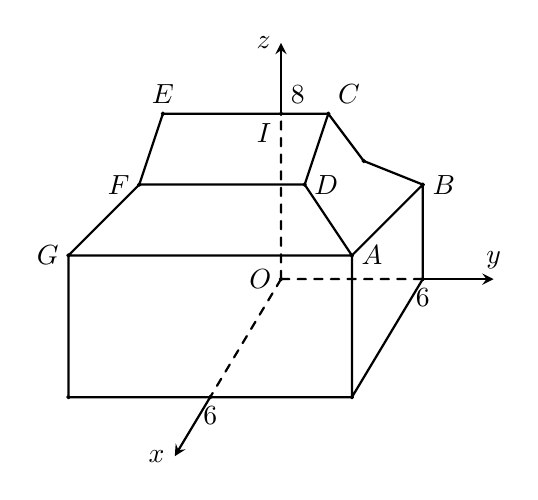
\begin{tikzpicture}[scale=0.3,line join=round,line cap=round,>=stealth]
            \coordinate (O) at (0,0);
            \draw[fill=black] (O) node[left]{$O$} circle (2pt);
            \coordinate (A) at (3,1);
            \draw[fill=black] (A) node[right]{$A$} circle (2pt);
            \coordinate (B) at (6,4);
            \draw[fill=black] (B) node[right]{$B$} circle (2pt);
            \coordinate (C) at (2,7);
            \draw[fill=black] (C) node[above right]{$C$} circle (2pt);
            \coordinate (D) at (1,4);
            \draw[fill=black] (D) node[right]{$D$} circle (2pt);
            \coordinate (E) at (-5,7);
            \draw[fill=black] (E) node[above]{$E$} circle (2pt);
            \coordinate (F) at (-6,4);
            \draw[fill=black] (F) node[left]{$F$} circle (2pt);
            \coordinate (G) at (-9,1);
            \draw[fill=black] (G) node[left]{$G$} circle (2pt);
            \coordinate (K) at (3.5,5);
            \draw[fill=black] (K) node[above right]{} circle (2pt);
            \coordinate (I) at (0,7);
            \draw[fill=black] (I) node[below left]{$I$} circle (2pt);
            \coordinate (G1) at (-9,-5);
            \draw[fill=black] (G1) node[below]{} circle (2pt);
            \coordinate (A1) at (3,-5);
            \draw[fill=black] (A1) node[below]{} circle (2pt);
            \coordinate (B1) at (6,0);
            \draw[fill=black] (B1) node[below]{$6$} circle (2pt);
            \coordinate (Q) at (-3,-5);
            \draw[fill=black] (Q) node[below]{$6$} circle (2pt);
            \node at (0,7) [above right] {$8$};
            \draw[thick] (A)--(B)--(K)--(C)--(D)--(A)--(G)--(F)--(D)
            (C)--(E)--(F)
            (G)--(G1)--(A1)--(A)
            (A1)--(B1)--(B);
            \draw[thick,dashed] (O)--(Q)
            (O)--(B1)
            (O)--(I);
            \draw[->,thick] (Q) -- (-4.5,-7.5) node[left] {$x$};
            \draw[->,thick] (6,0) -- (9,0) node[above] {$y$};
            \draw[->,thick] (0,7) -- (0,10) node[left] {$z$};
        \end{tikzpicture}
    \end{center}
    Giả sử áp dụng hệ trục toạ độ $Oxyz$ như hình vẽ (đơn vị trên các trục là mét). Xét một bên của mái nhà gồm có một hình chữ nhật $CDFE$ và một hình thang $ADFG$ với các điểm có toạ độ lần lượt là $G(6;-6;6)$, $C(3;4;8)$, $F(4;-4;7)$ và điểm $I$ là trung điểm $CE$. Biết góc giữa hai vectơ $\overrightarrow{DC}$ và $\overrightarrow{AB}$ bằng $a^{\circ}$. Giá trị của $a$ bằng bao nhiêu (\textit{làm tròn kết quả đến hàng đơn vị})?
    \par
    \shortans[0]{45}
    \loigiai{
        Từ hình vẽ ta tìm được $A(6;6;6)$ và hình chiếu của $A$ xuống $(Oxy)$ là $A'(6;6;0)$.\\ 
        Toạ độ điểm $B(0;6;6)$ và $D(4;4;7)$ nên do đó $\overrightarrow{DC}=(-1;0;1)$ và $\overrightarrow{AB}=(-6;0;0)$.\\ 
        Mặt khác $\cos \left(\overrightarrow{DC},\overrightarrow{AB}\right)=\dfrac{\overrightarrow{DC}\cdot \overrightarrow{AB}}{\left|\overrightarrow{DC}\right|\cdot \left|\overrightarrow{AB}\right|}=\dfrac{\sqrt{2}}{2}\Rightarrow a=45^{\circ}$.\\ 
        Vậy giá trị của $a$ bằng $45$.
    }
\end{ex}
\Closesolutionfile{ans}
%\inputansbox{5}{ans/DA-CD4-BTRL}